
\documentclass{report}
\usepackage{graphicx}
\usepackage{outlines}
\usepackage{multirow}
\usepackage{tabularx}
\usepackage{nameref}
\usepackage{hyperref}
\usepackage{listings}
\usepackage{titlepic}
\usepackage[margin=1in]{geometry}
\setcounter{secnumdepth}{5}
\setcounter{tocdepth}{5}

\hypersetup{%
	pdfborder = {0 0 0}
}

\makeatletter
\renewcommand\paragraph{\@startsection{paragraph}{4}{\z@}%
  {-3.25ex\@plus -1ex \@minus -.2ex}%
  {1.5ex \@plus .2ex}%
  {\normalfont\normalsize\bfseries}}
\renewcommand\subparagraph{\@startsection{subparagraph}{5}{\z@}%
  {-3.25ex\@plus -1ex \@minus -.2ex}%
  {1.5ex \@plus .2ex}%
  {\normalfont\normalsize\bfseries}}
\makeatother

\begin{document}

\title{AVM Component Model Specification Documentation\\Version 2, Draft 1}
\author{Adam Nagel\\
	Institute for Software Integrated Systems (ISIS)\\
	Vanderbilt University\\
	\texttt{adam@isis.vanderbilt.edu}\\
	\\
	Developed for the DARPA Adaptive Vehicle Make (AVM) Program}
\date{\today}
\titlepic{

\includegraphics[scale=0.75]{ISIS-logoNEW} \hspace{1cm}

\includegraphics[scale=0.103]{DARPA-logo}
}

\maketitle


\tableofcontents

\section{AVM Component Model Schema}
\label{AVM_Component_Model_Schema}

\subsection{Overview}
The \textbf{AVM Component Model} captures data and metadata about an AVM Component. From a system designer's perspective, it is a "black box," below which the designer does not need composition details.

An AVM Component Model serves several purposes: 
\begin{itemize}
\item Capture the metadata of the component, including information on its dependent artifacts
\item Define the interfaces and properties of the component for use in composing system models
\item Serve as a wrapper for integrating various domain models of the component
\end{itemize}

\subsection{Core Concepts}

\subsubsection{Properties and Parameters}
The core metadata about a component is expressed using properties and parameters. Properties represent attributes of a component that can not be directly altered by the user of a component, while Parameters represent designed variability of a component. The variability of a component can range from geometric  (e.g. dimensions of a parametrized fuel tank), to behavioral (e.g. gain constants of a PID controller), to interface variability (e.g. structural connector types).  

\begin{table}[H]
\begin{center}
\begin{tabular}{|l|l|l|l|l|}
\hline
 \textbf{Name} & \textbf{Value} & \textbf{Data Type} & \textbf{Unit} & \textbf{Dimensions}\\
 \hline
 efficiency & 0.85 & Real & N/A & 1  \\
 \hline
 case\_heat\_transfer\_area & 3.84 & Real & m\^2 & 1 \\
 \hline
\end{tabular}
\caption{Example Properties of an Engine Component}
\end{center}
\label{Properties_Table}
\end{table}

\begin{table}[H]
\begin{center}
\begin{tabular}{|l|l|l|l|l|l|l|}
\hline
 \textbf{Name} & \textbf{Def. Value} & \textbf{Min Value} & \textbf{Max Value} & \textbf{Data Type} & \textbf{Unit} & \textbf{Dimensions}\\
 \hline
 output\_mount\_position\_x & 1.0 & 0.4 & 10.0 & Real & N/A & 1  \\
 \hline
\end{tabular}
\caption{Example Parameters of a Parametric Drive Shaft}
\end{center}
\label{Parameters_Table}
\end{table}


\subsubsection{Connectors}
The AVM Component Specification allows multiple types of interfaces currently instantiated as Connectors and Ports. There are different types of Ports such as Power ports, Signal ports, and Structural ports. The Connectors are an aggregation of Ports. Connectors allow component designers to meaningfully group different Ports. For example, a power flow through a component will in most cases will require a physical interface, so it can be meaningfully represented with a Connector that aggregates a Power port, and a Structural port. When the component is used in a design, a single connection made with the Connector automatically and consistently results in the two separate Power and Structural connections. When individual Ports are used as interfaces it becomes the responsibility of the designer to ensure that connections are made in a consistent manner, and creates an implicit requirement from the component designer to the component user and is bound to result in problems. Therefore, the specification recommends usage of Connectors when ports need to be connected simultaneously. 

\begin{table}[H]
\begin{center}
\begin{tabular}{|l|l|l|p{5cm}|}
\hline
 \textbf{Connector Name} & \textbf{Connector Roles} & \textbf{Port Map} & \textbf{Type} \\
 \hline
 eng\_torque\_out & Z\_Axis & cad.EXT\_TORQUE\_OUT\_axis\_z & Axis  \\
  & YX\_Plane & cad.EXT\_TORQUE\_OUT\_plane\_xy & Plane  \\
  & YZ\_Plane & cad.EXT\_TORQUE\_OUT\_plane\_yz & Plane \\
  & brg\_02 & mod.conn\_brg\_02 & Modelica.Mechanics.Multibody.
  Interfaces.FlangeWithBearing  \\
 \hline
\end{tabular}
\caption{Example Connector of an Engine Component}
\end{center}
\label{Properties_Table}
\end{table}

\subsubsection{Domain Model Sublanguage}
A \textbf{Domain Model} is a domain-specific model that describes the component in that domain. Examples of these include CAD models, Modelica behavioral models, cyber models, manufacturing models, and more.

Each \textbf{Domain Model} may include instantiations of \textbf{Ports}, \textbf{Parameters}, and \textbf{Metrics}. \textbf{Ports} are composition points specific to the domain. \textbf{Parameters} are variables of the domain model that may be set prior to the model's use in a composition (simulation, geometric model, etc). \textbf{Metrics} are variables that may be checked after a model's use in a composition (mass calculation from a parametric CAD model, max force in a physics simulation, etc).

Domain-specific models are defined as \textit{extensions} of the abstract \textit{DomainModel} baseclass. Composition points are modeled as extensions of the \textit{DomainModelPort} abstract baseclass, and likewise with Parameters and Metrics. They are typically defined within tool-specific namespaces to avoid name collisions (e.g.: \textit{avm.cad}, \textit{avm.modelica}).

Current examples include ModelicaModel, CADModel, CyberModel, and ManufacturingModel, although the spec is extensible to include more domains.

\label{Domain_Model_Alternatives}
If more than one of a given class of DomainModel is included in the Component package, then these models are considered to be \textit{alternative} representations of the complete component. These representations may vary in fidelity or suitability for a specific type of analysis.

When performing an analysis, users will select between alternative Domain Models by inspecting the Name field.

\subsubsection{Composition Semantics}
\label{Composition_Semantics}
Components are designed to be composed with other components via their \textbf{Connectors}. When two component connectors are composed, then their corresponding \textbf{Role} elements are also matched, and the \textbf{DomainPorts} so mapped will be connected together in a generated domain model.

In the example given in \textbf{Figure \ref{Composition_Example}}, two components each have embedded Domain Models of type \textbf{ModelicaModel}. They also each feature \textbf{Connector} objects that share a common definition. The \textbf{role} objects within each \textbf{connector} instance are mapped to the \textbf{modelica connectors} of each component's Modelica model. In the generated Modelica model, the corresponding Modelica class representing each component is instantiated, and their connectors are joined by following the \textit{ Modelica Connector$\rightarrow$Role$\rightarrow$Connector$\rightarrow$Connector$\rightarrow$Role$\rightarrow$Modelica Connector} chain from the source AVM META composition.

\begin{figure}
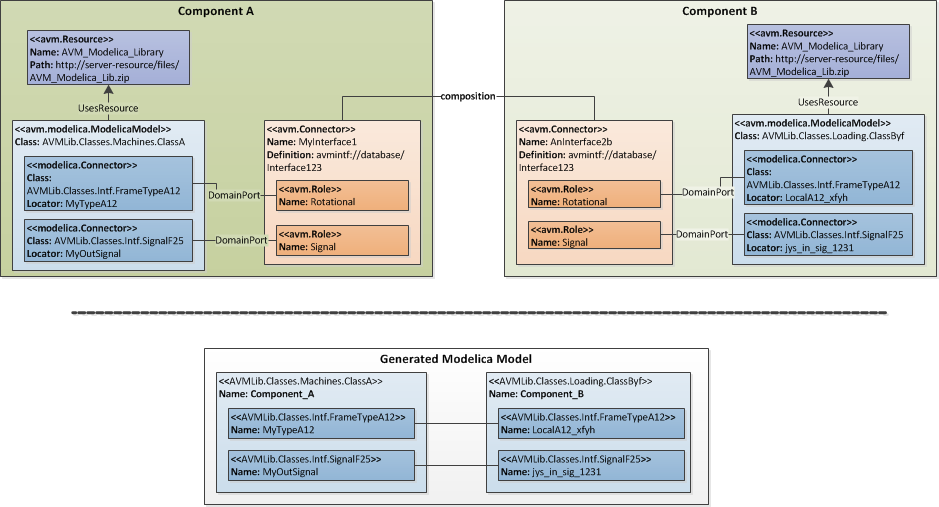
\includegraphics[width=\textwidth]{CompositionExample}
\caption{Example illustrating composition semantics. At top, the composition of two Component models within an AVM META design tool. At bottom, the resulting composition within a Modelica model generated by those tools.}
\label{Composition_Example}
\end{figure}

\subsubsection{Value Sublanguage}
The specification includes a sublanguage for expressing values, as seen in the "Values" ClassDiagram (see Figure \ref{Value_diagram}). Within components, many elements have values, and these values may be fixed, derived from other sources, parametrically variable by the user, or probabilistic. This sublanguage for expressing values allows a high degree of flexibility in establishing dependent relationships between values in a model.

Each \textbf{Value} container contains a characterization of its unit (e.g., meter, mph), datatype (e.g., integer, boolean), and dimensionality (e.g., scalar, vector, matrix). The Value container then contains one \textbf{ValueExpression}, which describes how the value should be determined. There are several variations, including fixed, calculated, derived, parametric, and probabilistic. For many of these, key attributes may themselves be expressed using ValueExpressions.


\subsection{Implementation}
\subsubsection{File Format}
AVM Component Models are stored in files with an extension of .ACM. Their contents are in XML format. An XML schema (in XSD format) enforces the syntax of the spec.


\subsubsection{Software Library}
\label{ACMAPI}
The AVM Component Model is also supported by software libraries that can parse, validate, and export AVM Component Models. These libraries provide classes specific to AVM Component concepts.

\begin{itemize}
\item \textbf{Python}
An initial library implementation in Python is provided. It was generated using \textbf{PyXB}, a tool which generates Python classes from an XML Schema.

An example model-building program is provided (\textit{test\_builder.py}).

\item \textbf{Java}
An initial library implementation in Java is provided. It was generated using \textbf{JAXB}, a tool which generates Java classes from an XML Schema.

\item \textbf{C\# for .NET}
An implementation in C\#, for use with the .NET framework, is provided. It was generated using \textbf{Xsd2Code}, a tool which generates C\# classes from an XML Schema.

\end{itemize}

\subsubsection{Schema}
\label{ACMSchema}
An XML Schema file is provided for checking conformance to the ACM file format.

\subsubsection{Extending the ACM Format}
Although the AVM Component Model format was designed to be extensible, the schema does not yet support the use of new tags. A set of best practices for extending the format remains to be defined.

\subsection{Classes}
This section documents and provides detail description of different classes in the AVM component model schema. The classes are organized in multiple namespaces to avoid name collisions. The core concepts that apply to the component are included in the \textbf{avm} namespace, while concepts relevant to domain model wrappers are included in the \textbf{cad, modelica, cyber, and manufacturing} namespaces respectively.

\subsubsection{avm Namespace}
The classes in avm Namespace are described below, and their relations are depicted in class diagrams in figures below.

\begin{figure}[h!]
\fbox{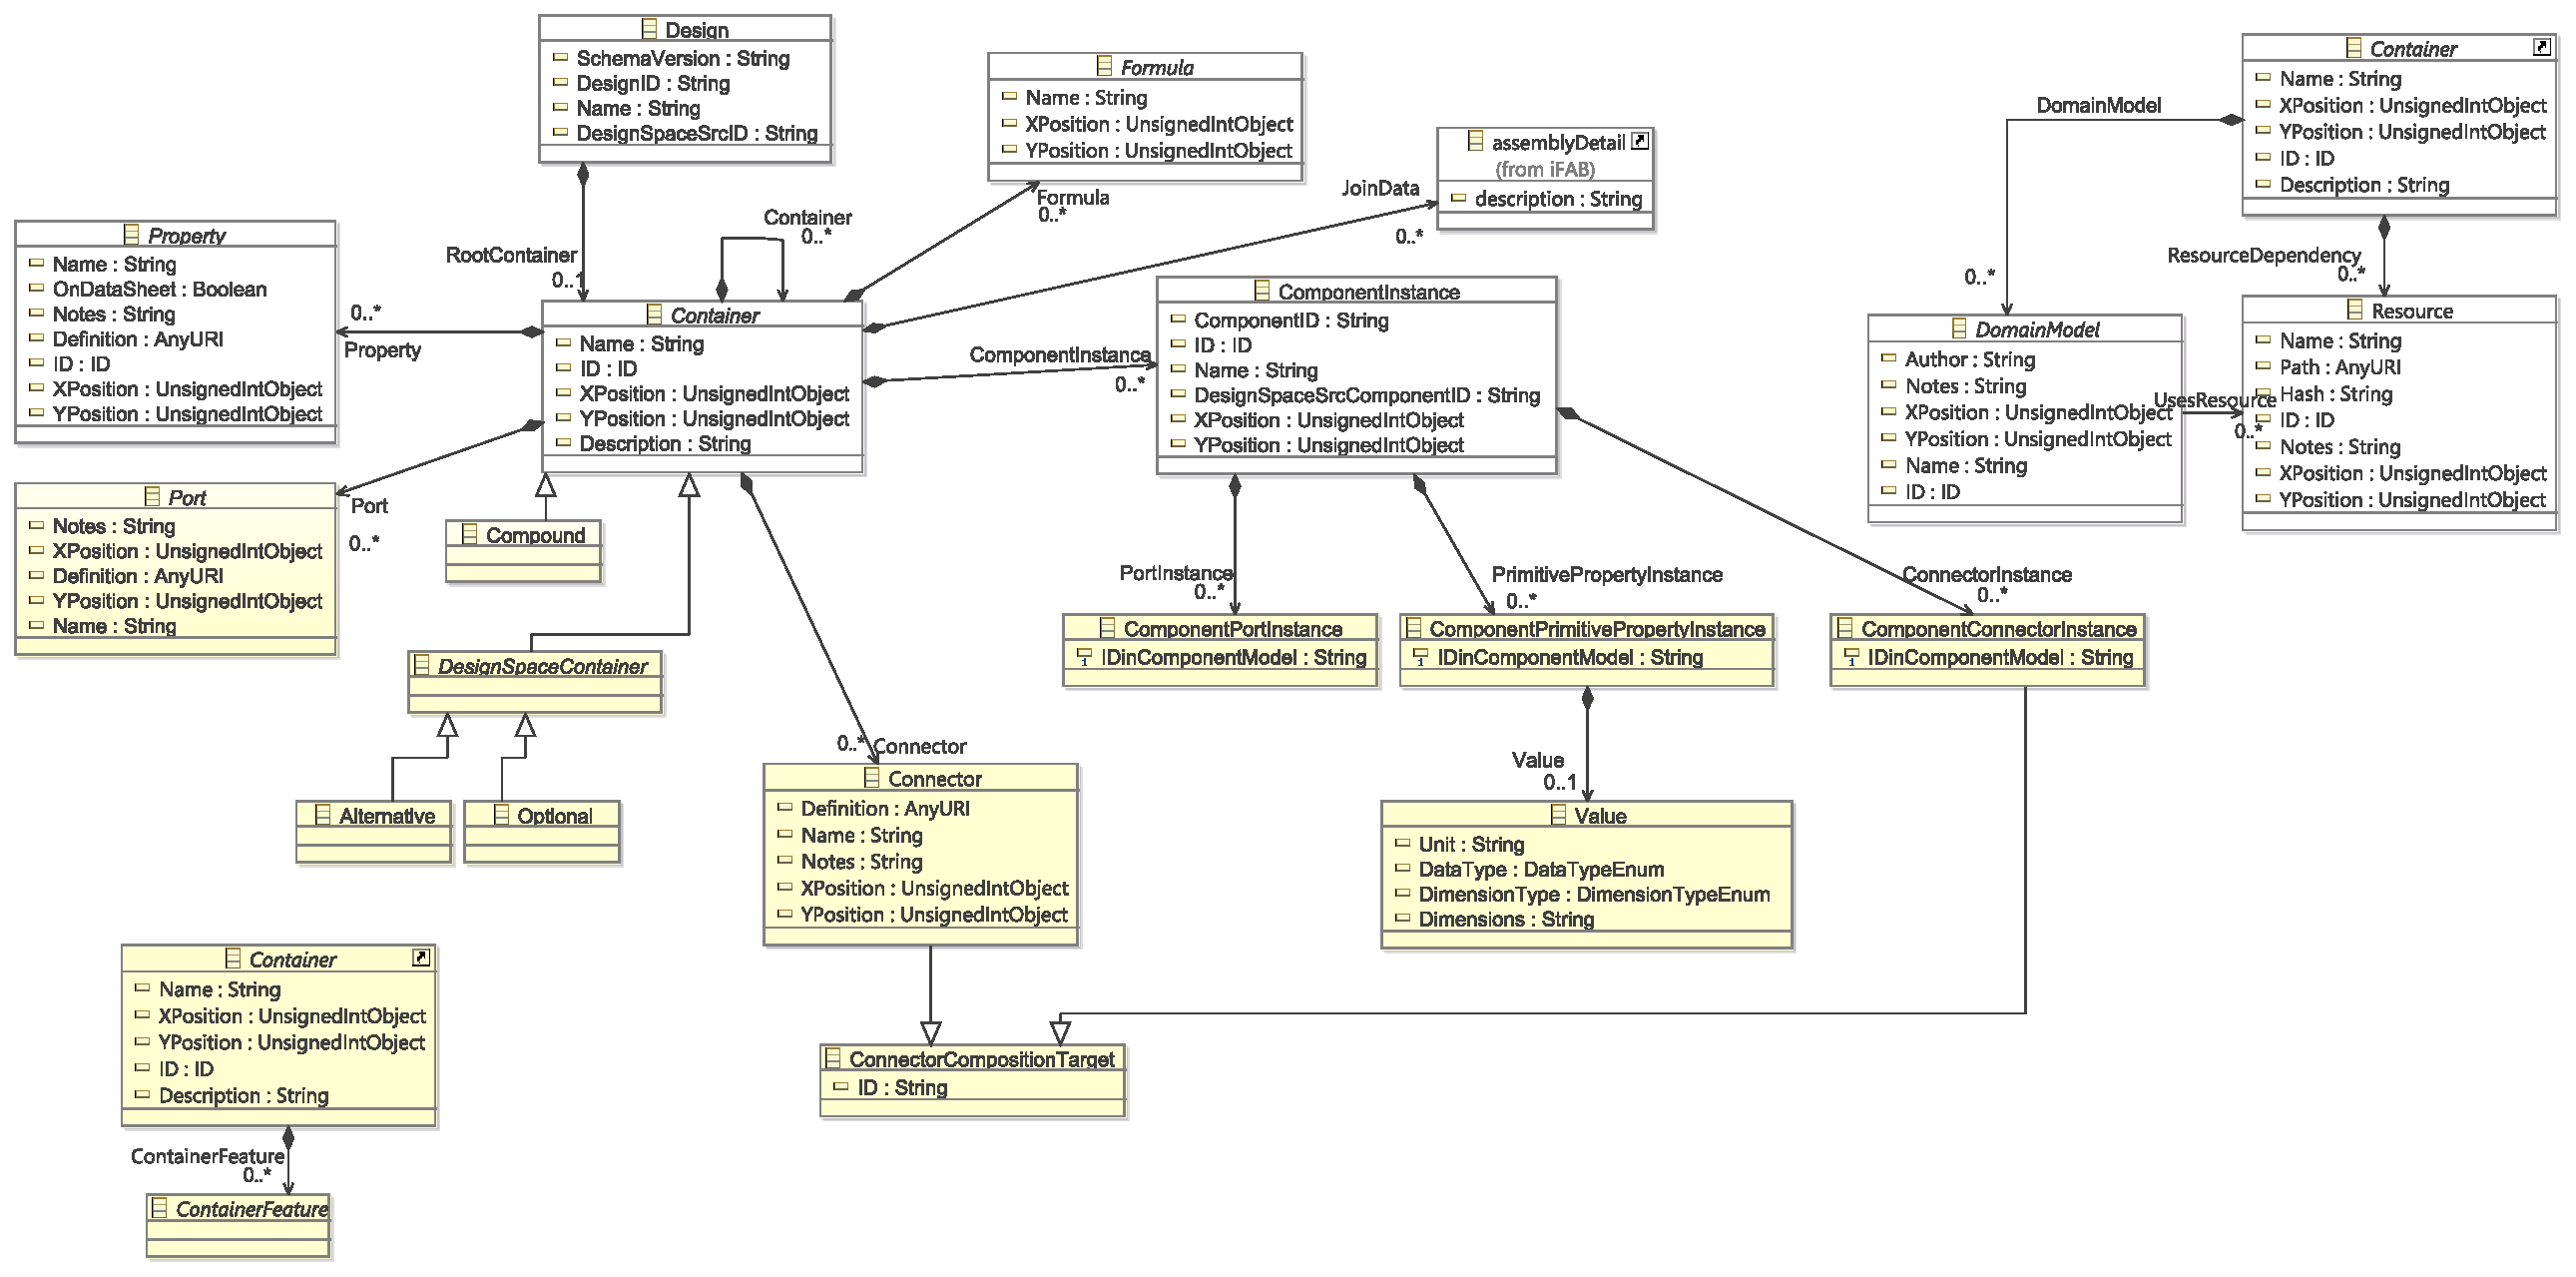
\includegraphics[width=\textwidth]{ClassDiagrams/avm_design.pdf}}
\caption{avm Namespace: Design diagram}
\label{Design_Diagram}
\end{figure}


\paragraph{avm.Component}
{\bf Component} is the root element of an AVM Component definition.
\\ \\
\begin{tabular}{ l l p{12cm} }
\textbf{Attribute} & \textbf{Type} & \textbf{Description} \\ \hline
Name & String & The name of the component\\ \hline
Version & String & The version number for the component\\ \hline
SchemaVersion & String & The version of the AVM Component schema to which this component conforms\\ \hline
ID & String & A string that uniquely identifies this Component model\\ \hline
Classifications & AnyURI[] & A list of URIs that identify classes to which this component belongs.\\ \hline
Supercedes & String[] & A list of IDs of Components that this component supercedes (is a newer version of).
\end{tabular}


\DefineVerbatimEnvironment%
  {MyVerbatim}{Verbatim}
  {frame=single,fontfamily=courier}
\begin{MyVerbatim}
<ns1:Component 
    xmlns:ns1="avm" xmlns:ns2="manufacturing" 
    xmlns:ns3="modelica" xmlns:ns4="cad" 
    xmlns:xsi="http://www.w3.org/2001/XMLSchema-instance" 
  Name="engine_compression_ignition_diesel__cat__c9_600hp" 
  Version="10_10_2013_17_23"
  SchemaVersion="1.0"
  ID="AVM.Component.2e61b1472b"  >
    <Classifications>Engine_Compression_Ignition_Diesel</Classifications>
    ...
</ns1:Component>
\end{MyVerbatim}

\paragraph{avm.DistributionRestriction}
\textit{(Abstract)} Baseclass for a number of expressions that describe distribution restrictions that apply to the component.
\\ \\
\begin{tabular}{ l l p{12.5cm} }
\textbf{Attribute} & \textbf{Type} & \textbf{Description} \\ \hline
Note & String & A note providing details of the restriction. \\ \hline
\end{tabular}

\paragraph{avm.SecurityClassification}
\textit{Subtype of avm.DistributionRestriction}\\
Describes a security classification that applies to the component. If no SecurityClassification element is found, the component is assumed to be unclassified.
\\ \\
\begin{tabular}{ l l p{12.5cm} }
\textbf{Attribute} & \textbf{Type} & \textbf{Description} \\ \hline
Level & String & The classification level that applies \\ \hline
\end{tabular}

\paragraph{avm.Proprietary}
\textit{Subtype of avm.DistributionRestriction}\\
Describes an organization that claims this component as proprietary.
\\ \\
\begin{tabular}{ l l p{12.5cm} }
\textbf{Attribute} & \textbf{Type} & \textbf{Description} \\ \hline
Organization & String & (Required) The organization claiming that the component is proprietary. \\ \hline
\end{tabular}

\begin{MyVerbatim}[frame=single]
  <DistributionRestriction Organization="Ricardo Inc"
     xsi:type="ns1:Proprietary"/>
\end{MyVerbatim}

\paragraph{avm.ITAR}
\textit{Subtype of avm.DistributionRestriction}\\
Describes an ITAR restriction that applies to this component. If this ITAR element is found, the component is assumed to be ITAR. If no ITAR element is are found, the component is assumed to be non-ITAR.

\begin{MyVerbatim}[frame=single]
  <DistributionRestriction Level="ITAR" xsi:type="ns1:ITAR" 
Notes="Notes about this ITAR restriction."/>
\end{MyVerbatim}

\paragraph{avm.DoDDistributionStatement}
\textit{Subtype of avm.DistributionRestriction}\\
Describes a Department of Defense (DoD) distribution statement that applies to this component.
\\ \\
\begin{tabular}{ l l p{9cm} }
\textbf{Attribute} & \textbf{Type} & \textbf{Description} \\ \hline
Type & DoDDistributionStatementEnum & (Required) The DoD distribution statement that applies to this component. \\ \hline
\end{tabular}


\begin{figure}[h!]
\fbox{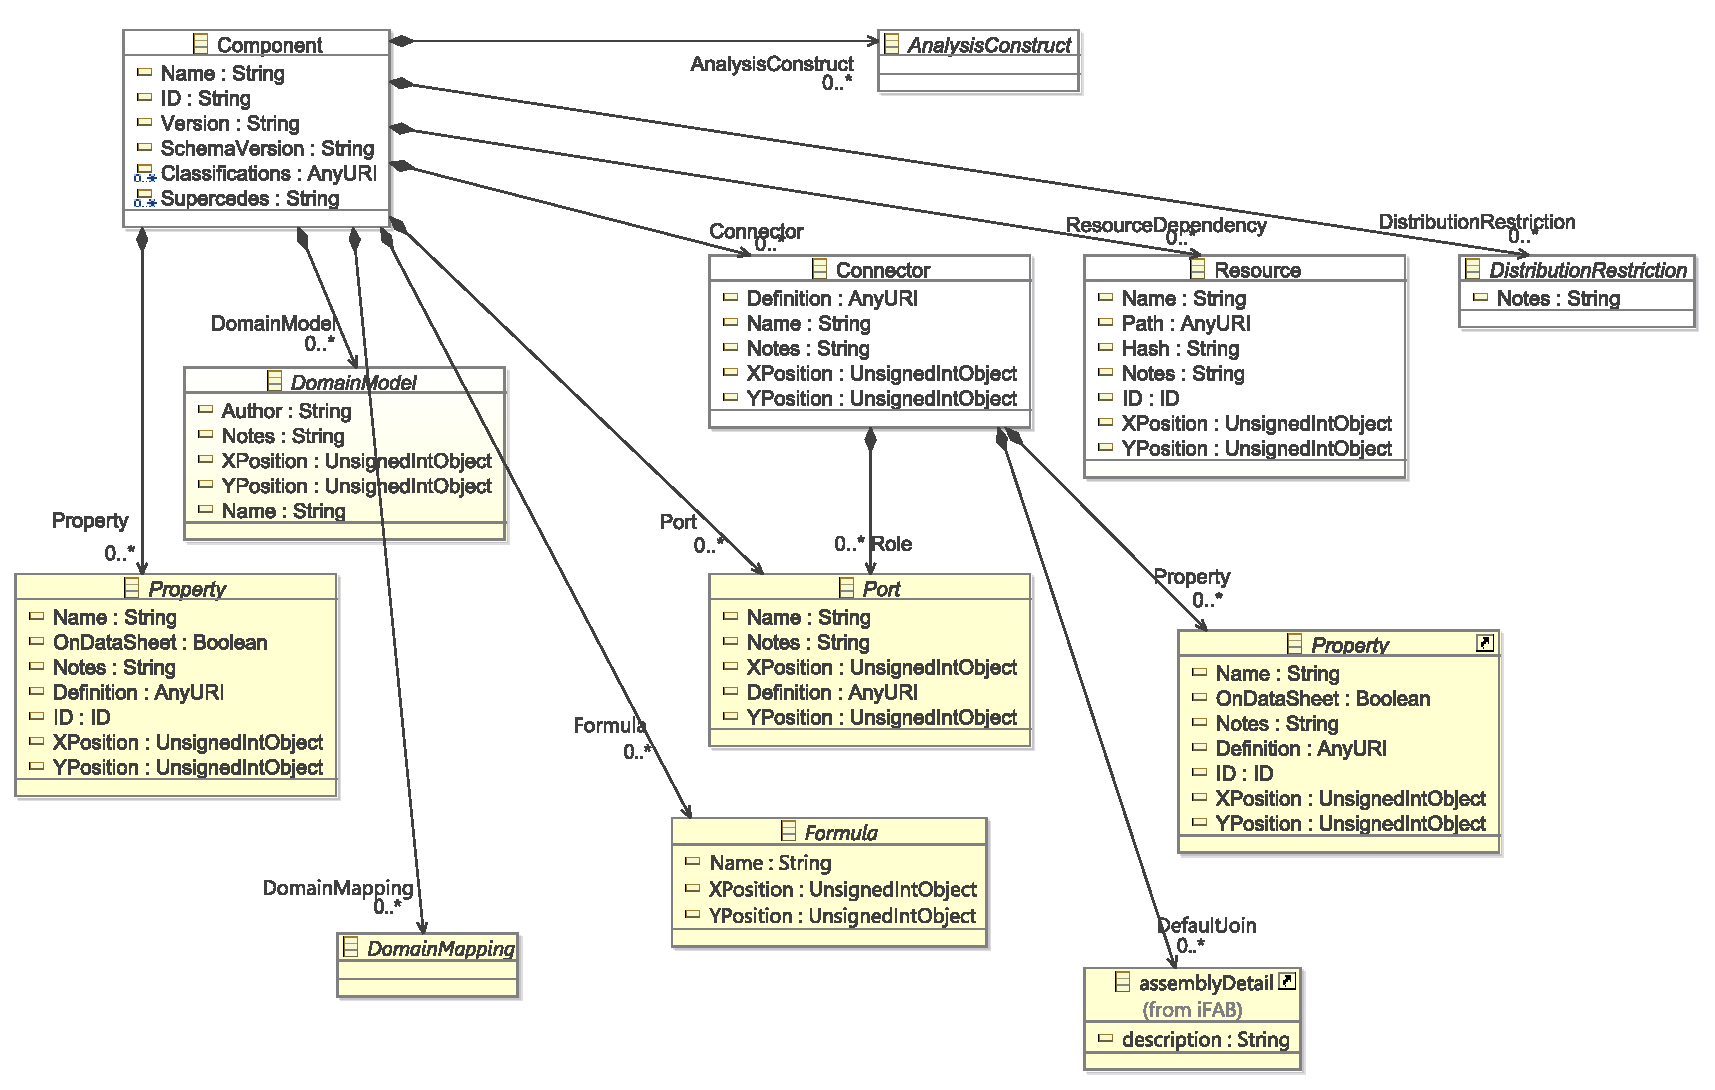
\includegraphics[width=\textwidth]{ClassDiagrams/avm_component.pdf}}
\caption{avm Namespace: Component diagram}
\label{Component_diagram}
\end{figure}

\begin{figure}[h!]
\fbox{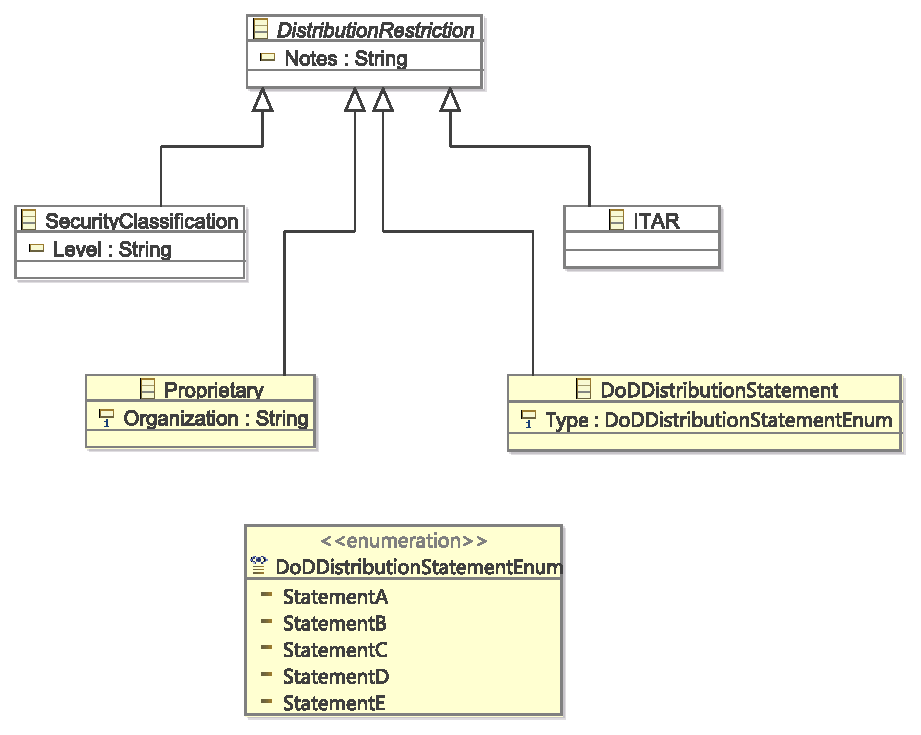
\includegraphics[width=\textwidth]{ClassDiagrams/avm_distributionrestrictions.pdf}}
\caption{avm Namespace: Distributionrestrictions diagram}
\label{Restriction_diagram}
\end{figure}

\paragraph{avm.Property}
\textit{(Abstract)} Captures a property of a component. When instantiated into a component, it may have a fixed value, have a value described by a probability distribution, be parametrically variable at design time, or be derived from other values.
\\ \\
\begin{tabular}{ l l p{12cm} }
\textbf{Attribute} & \textbf{Type} & \textbf{Description} \\ \hline
Definition & AnyURI & If this property is strongly typed and instantiated from a definition database, this is its definition URI \\ \hline
Name & String & The name of the property, as instantiated \\ \hline
OnDataSheet & Boolean & Selects whether this property should be prominently displayed on "data sheet"-style views of the component \\ \hline
Notes & String & Any notes describing the property \\ \hline
ID & ID & The ID of this property, unique within the scope of the component model \\ \hline
\end{tabular}

\paragraph{avm.PrimitiveProperty}
A property that is described by a value.
\\ \\
\begin{tabular}{ l l p{6cm} }
\textbf{Relation} & \textbf{Type} & \textbf{Description} \\ \hline
Value & Value & The Value container for this property \\ \hline
\end{tabular}

\begin{MyVerbatim}[frame=single]
  <Property   
    Definition="CML_Physical_Quantity\cml_zodb.cml_basic_physicals.Efficiency"
   ID="primitive.cac_performance" Name="cac_performance" 
   xsi:type="ns1:PrimitiveProperty">
    <Value>
      ...
    </Value>
  </Property>
\end{MyVerbatim}

\paragraph{avm.CompoundProperty}
A property that is a container for other properties.
\\ \\
\begin{tabular}{ l l p{9cm} }
\textbf{Relation} & \textbf{Type} & \textbf{Description} \\ \hline
PrimitiveProperty & PrimitiveProperty & Primitive Property children of this Compound Property \\ \hline
CompoundProperty & CompoundProperty & Compound Property children of this Compound Property \\ \hline
\end{tabular}

\begin{MyVerbatim}[frame=single]
 <Property Definition="CML_Mapping\cml_zodb.cml_component.CML_Common_Info" 
   ID="compound.common_info" Name="common_info" 
   xsi:type="ns1:CompoundProperty">
    <CompoundProperty 
    Definition="CML_Mapping\cml_zodb.cml_extended_physicals.Bounding_Box" 
    ID="compound.common_info.overall_dimensions" 
    Name="overall_dimensions">
      <PrimitiveProperty 
        Definition="CML_Physical_Quantity\cml_zodb.cml_basic_physicals.Length" 
        ID="primitive.common_info.overall_dimensions.height" 
        Name="height">
        <Value>...</Value>
      </PrimitiveProperty>
      <PrimitiveProperty   
        Definition="CML_Physical_Quantity\cml_zodb.cml_basic_physicals.Length" 
        ID="primitive.common_info.overall_dimensions.length"
        Name="length">
        <Value>...</Value>
      </PrimitiveProperty>
      <PrimitiveProperty 
        Definition="CML_Physical_Quantity\cml_zodb.cml_basic_physicals.Length" 
        ID="primitive.common_info.overall_dimensions.width" 
        Name="width">
        <Value>...</Value>
      </PrimitiveProperty>
    </CompoundProperty>
\end{MyVerbatim}

\begin{figure}[h!]
\fbox{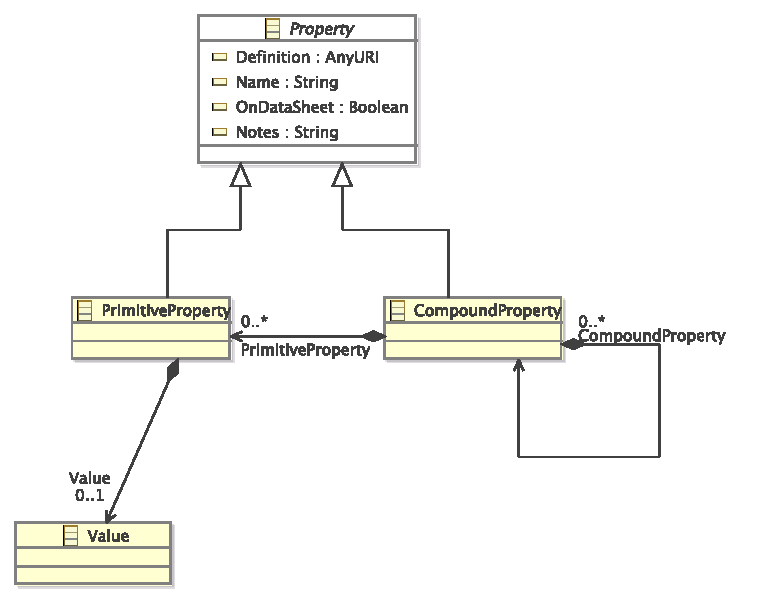
\includegraphics[width=\textwidth]{ClassDiagrams/avm_property.pdf}}
\caption{avm Namespace: Property diagram}
\label{Property_diagram}
\end{figure}

\paragraph{avm.ValueNode}
Abstract baseclass representing an object that carries a value, whether as a Value or Formula object.
\\ \\ 
\begin{tabular}{ l l p{9.5cm} }
\textbf{Attribute} & \textbf{Type} & \textbf{Description} \\ \hline
ID & String & (required) An ID, unique within the scope of the component model, used for referring to this value container. \\ \hline
\end{tabular}

\paragraph{avm.Formula}
Abstract baseclass representing an object that describes a calculation. The result of the calculation must be passed to any \textbf{DerivedValue} object that has this calculation as a \textit{ValueSource}, or to any \textbf{Formula} that has this calculation as an \textit{Operand}.
\\ \\
\begin{tabular}{ l l p{9.5cm} }
\textbf{Attribute} & \textbf{Type} & \textbf{Description} \\ \hline
Name & String & The Name of the formula. \\ \hline
XPosition & Unsigned Int & The X Position of the element, if rendered graphically within its parent model \\ \hline
YPosition & Unsigned Int & The Y Position of the element, if rendered graphically within its parent model \\ \hline
\end{tabular}

\paragraph{avm.SimpleFormula}
A \textbf{SimpleFormula} represents a basic calculation. A number of \textbf{ValueNode} objects serve as operands, with the operation determined by the \textit{Operation} attribute.
\\ \\
\begin{tabular}{ l l p{9.5cm} }
\textbf{Attribute} & \textbf{Type} & \textbf{Description} \\ \hline
Operation & SimpleFormulaOperation & The operation to be performed on the operands. \\ \hline
\end{tabular}
\\ \\ \\
\begin{tabular}{ l l p{10cm} }
\textbf{Relation} & \textbf{Type} & \textbf{Description} \\ \hline
Operand & ValueNode & A ValueNode that will serve as an operand to the calculation. \\ \hline
\end{tabular}

\paragraph{avm.ComplexFormula}
A \textbf{ComplexFormula} represents a calculation described by an \textit{Expression}.
\\ \\
\begin{tabular}{ l l p{9.5cm} }
\textbf{Attribute} & \textbf{Type} & \textbf{Description} \\ \hline
Expression & String & The expression to be evaluated with the included operands. Must obey \textsc{\nameref{subsec:ComplexFormulaExpressionSyntax}}. The result of this expression will be calculated and considered the value of this \textbf{ValueNode}, so no assigment operator is required.\\ \hline
\end{tabular}
\\ \\ \\
\begin{tabular}{ l l p{10cm} }
\textbf{Relation} & \textbf{Type} & \textbf{Description} \\ \hline
Operand & Operand & A symbol and ValueSource that represents an operand of the expression \\ \hline
\end{tabular}

\paragraph{avm.Operand}
An \textbf{Operand} represents a symbol and value to be used in a \textbf{ComplexFormula} expression.
\\ \\
\begin{tabular}{ l l p{9.5cm} }
\textbf{Attribute} & \textbf{Type} & \textbf{Description} \\ \hline
Symbol & String & The symbol for the operand. The \textbf{ComplexFormula} \textit{Expression} will refer to this value by its symbol. The symbol must not start with a number or include any spaces or mathematical operators. \\ \hline
\end{tabular}
\\ \\ \\
\begin{tabular}{ l l p{10cm} }
\textbf{Relation} & \textbf{Type} & \textbf{Description} \\ \hline
ValueSource & ValueNode & The node from which the value for this operand should be taken. \\ \hline
\end{tabular}




\paragraph{avm.Value}
A \textbf{Value} container characterizes the nature of a value but not its exact expression. It may have one \nameref{ValueExpressionType} object as a child.
\\ \\
\begin{tabular}{ l l p{9.5cm} }
\textbf{Attribute} & \textbf{Type} & \textbf{Description} \\ \hline
Unit & String & The unit of the Value, expressed as the "symbol" specified by the QUDT unit library. \\ \hline
DataType & DataTypeEnum & Indicates the computing data type of the value. \\ \hline
DimensionType & DimensionTypeEnum & Indicates the dimension type of the value. \\ \hline
Dimensions & String & If DimensionType is non-scalar, indicates the dimensions of the data structure. \\ \hline
\end{tabular}

\begin{MyVerbatim}[frame=single]
    <Value 
      DataType="Real" 
      DimensionType="Scalar" 
      Dimensions="1" 
      ID="nv.case_thermal_conductivity" 
      Unit="W/(K*m)">
    ...
    </Value>
\end{MyVerbatim}

\paragraph{avm.ValueExpressionType}
\label{ValueExpressionType}
Abstract baseclass covering many types of expressions of the value.

\paragraph{avm.FixedValue}
With \textbf{FixedValue}, the value expression is captured as a string literal. Vectors and Matrices should be expressed using Python syntax.
\\ \\
\begin{tabular}{ l l p{7cm} }
\textbf{Attribute} & \textbf{Type} & \textbf{Description} \\ \hline
Value & String & A literal capturing the expressed value \\ \hline
\end{tabular}

\begin{MyVerbatim}[frame=single]
     <ValueExpression xsi:type="ns1:FixedValue">
        <Value>42.0</Value>
     </ValueExpression>
\end{MyVerbatim}

\paragraph{avm.CalculatedValue}
With \textbf{CalculatedValue}, the value expression is determined by executing a calculation or procedural code fragment (in Python). These expressions may use other available Value objects. The syntax for these expressions is not yet defined.
\\ \\
\begin{tabular}{ l l p{10cm} }
\textbf{Attribute} & \textbf{Type} & \textbf{Description} \\ \hline
Expression & String & (required) A declarative or procedural expression describing how the value should be determined \\ \hline
Type & CalculationTypeEnum & (required) Defines the type of the expression \\ \hline
\end{tabular}

\paragraph{avm.DerivedValue}
With \textbf{DerivedValue}, the value expression can be described as the value of another value container.
\\ \\
\begin{tabular}{ l l p{12.5cm} }
\textbf{Relation} & \textbf{Type} & \textbf{Description} \\ \hline
ValueSource & ValueNode & (required) The value container from which the value for this should be taken \\ \hline
\end{tabular}

\begin{MyVerbatim}[frame=single]
  <ValueExpression 
    ValueSource="nv.temp_inlet_nom_coolant" 
    xsi:type="ns1:DerivedValue"/>
\end{MyVerbatim}

\paragraph{avm.ParametricValue}
With \textbf{ParametricValue}, the value expression may be selected by a user of the component. For instance, a Component model may represent a driveshaft design with a parametrizable length, bounded by the limits of manufacturability. In this case, a user would select a driveshaft length when instantiating the component into their design.

Note that the attributes of this Value are themselves described with ValueExpressionType objects, making them flexible.
\\ \\
\begin{tabular}{ l l p{10cm} }
\textbf{Relation} & \textbf{Type} & \textbf{Description} \\ \hline
Default & ValueExpressionType & (required) The default value for this field. Used if no AssignedValue is provided. \\ \hline
AssignedValue & ValueExpressionType & The value that the user has assigned (overriding the default) \\ \hline
Minimum & ValueExpressionType & The minimum selectable value (if value must be a scalar number) \\ \hline
Maximum & ValueExpressionType & The maximum selectable value (if value must be a scalar number)) \\ \hline
\end{tabular}

\paragraph{avm.ProbabilisticValue}
(Abstract) The value is described by a distribution.

\paragraph{avm.NormalDistribution}
The value is described by a normal distribution. Note that the parameters of the distribution are themselves described with ValueExpressionType objects, making them flexible.
\\ \\
\begin{tabular}{ l l p{9cm} }
\textbf{Relation} & \textbf{Type} & \textbf{Description} \\ \hline
Mean & ValueExpressionType & (required) The mean of the distribution \\ \hline
StandardDeviation & ValueExpressionType & (required) The standard deviation of the distribution \\ \hline
\end{tabular}

\paragraph{avm.UniformDistribution}
The value is described by a uniform distribution.

\begin{figure}[h!]
\fbox{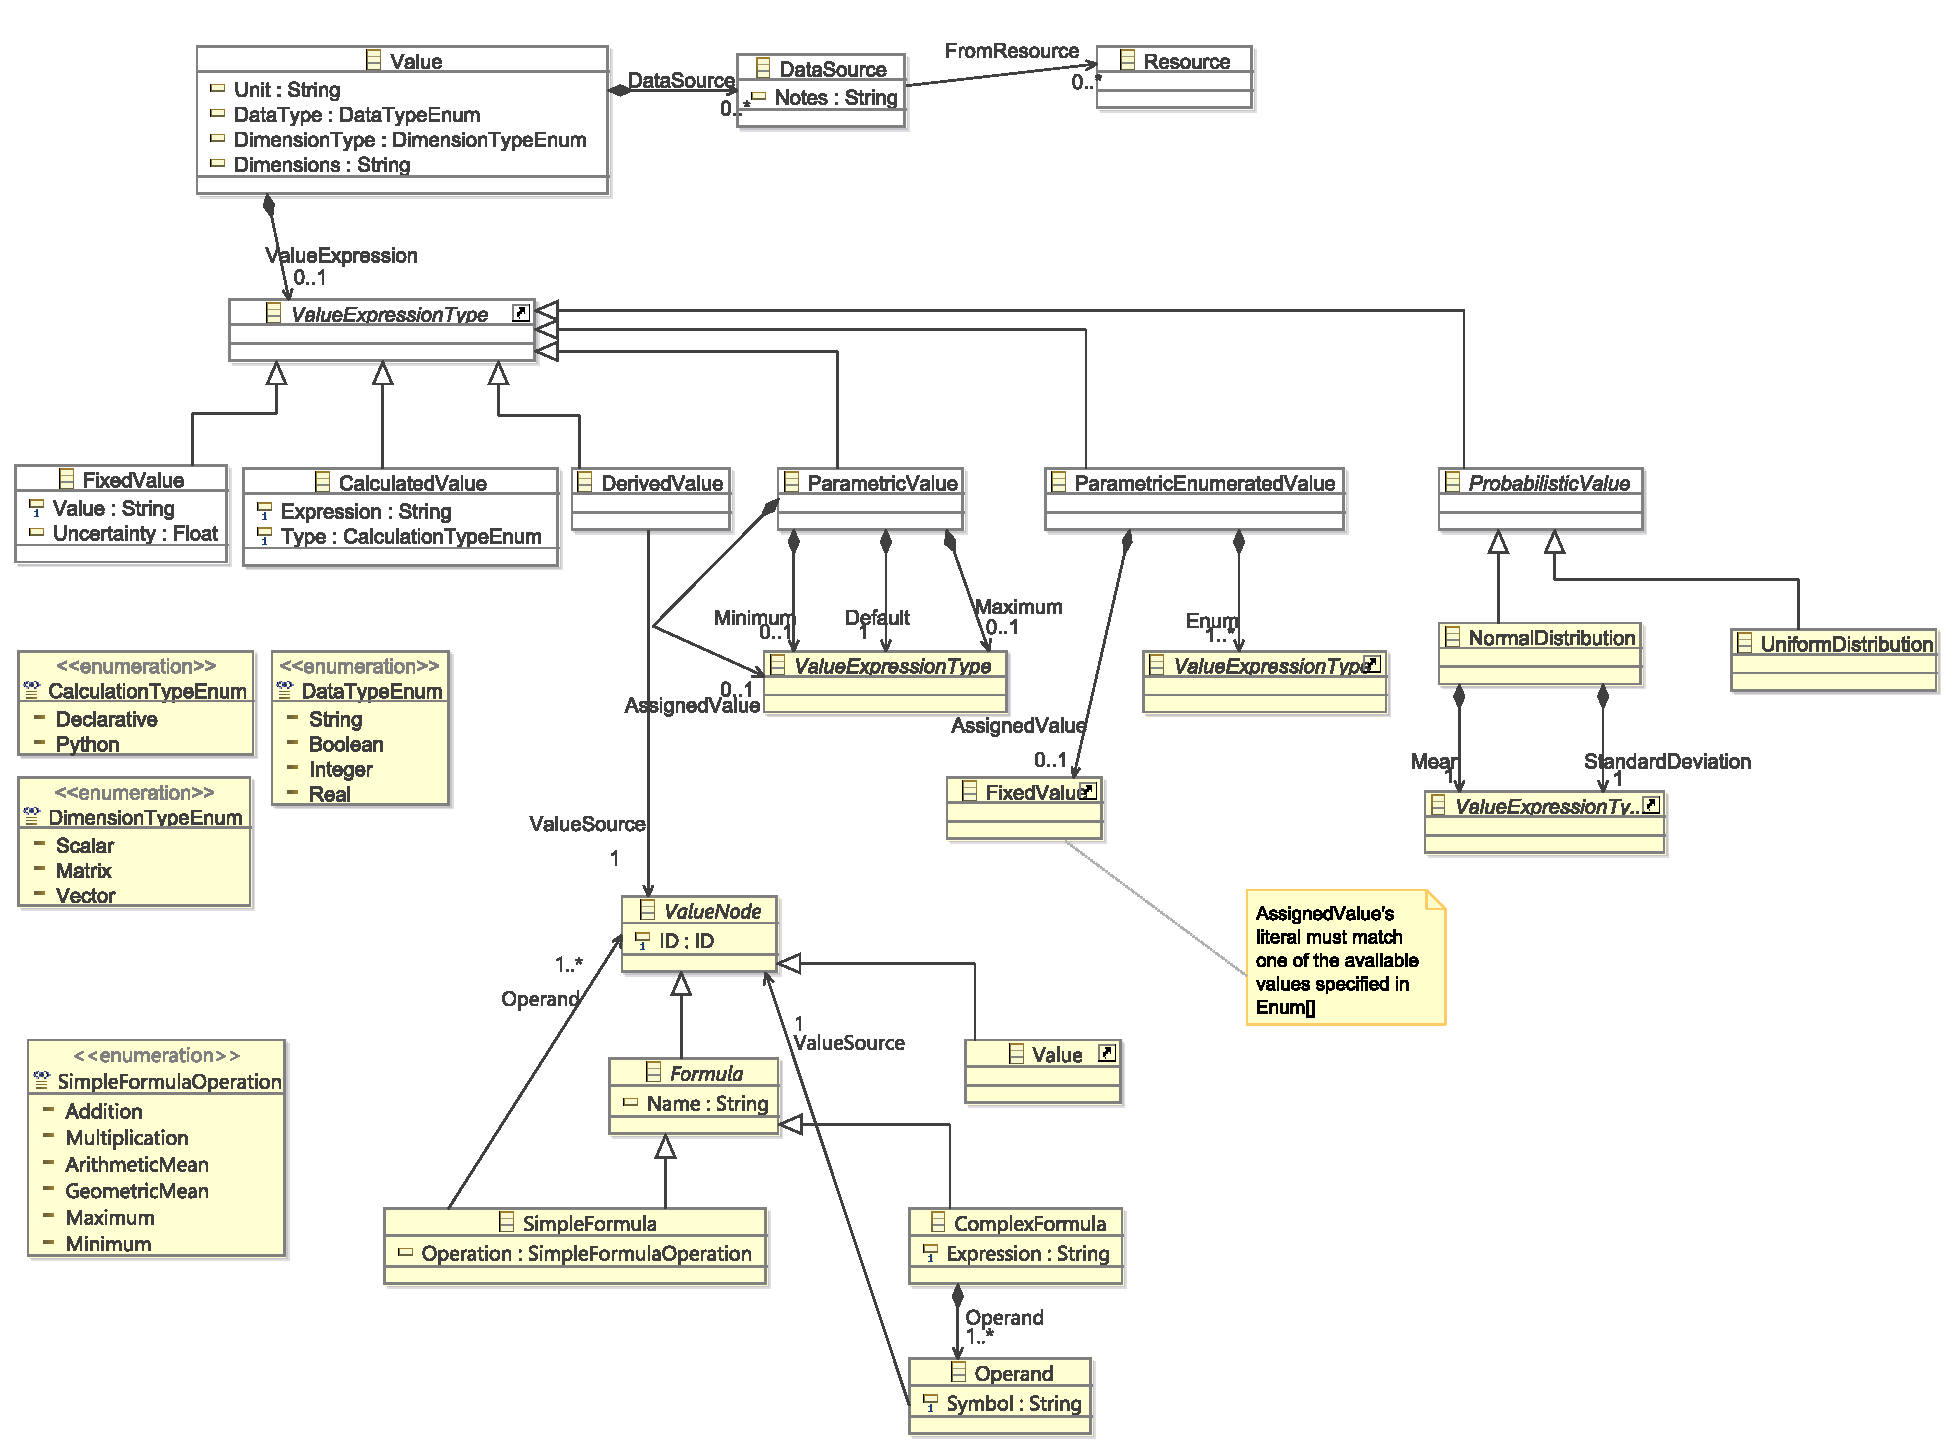
\includegraphics[width=\textwidth]{ClassDiagrams/avm_value.pdf}}
\caption{avm Namespace: Value diagram}
\label{Value_diagram}
\end{figure}


\paragraph{avm.Connector}
A Connector is an aggregation of DomainModelPort concepts that are intended to be composed at the same time. In a design context, the Connector is composed with another components's Connector, and the two Connectors must share a common definition.
See \ref{Composition_Semantics} for further discussion on Connector semantics.
\\ \\
\begin{tabular}{ l l p{12cm} }
\textbf{Attribute} & \textbf{Type} & \textbf{Description} \\ \hline
Definition & AnyURI & If this connector is strongly typed and instantiated from a definition database, this is its definition URI\\ \hline
Name & String & The name of this connector instance \\ \hline
Notes & String & Any notes describing the connector \\ \hline
XPosition & Unsigned Int & The X Position of the element, if rendered graphically within its parent model \\ \hline
YPosition & Unsigned Int & The Y Position of the element, if rendered graphically within its parent model \\ \hline
\end{tabular}
\\ \\ \\
\begin{tabular}{ l l p{12cm} }
\textbf{Relation} & \textbf{Type} & \textbf{Description} \\ \hline
Role & Port & Ports that are members of the Connector. These Ports must be mapped to DomainModelPorts contained within DomainModels of the Component. \\ \hline
\end{tabular}

\begin{MyVerbatim}
  <Connector 
    ConnectorComposition="cml_zodb.cml_connectors_mechanical.
      CML_Connector_Mechanical_Shaft_Spline_Involute" 
    ID="conn.eng_torque_out_to_transmission" 
    Name="eng_torque_out_to_transmission">
    <Role Name="Z_Axis" PortMap="cad.EXT_TORQUE_OUT_axis_z"      
      xsi:type="ns4:Axis"/>
    <Role Name="XY_Plane" PortMap="cad.EXT_TORQUE_OUT_plane_xy" 
      xsi:type="ns4:Plane"/>
    <Role Name="YZ_Plane" PortMap="cad.EXT_TORQUE_OUT_plane_yz" 
      xsi:type="ns4:Plane"/>
    <Role Class="Modelica.Mechanics.MultiBody.Interfaces.FlangeWithBearing" 
      Name="brg_02" PortMap="mod.conn.brg_02" xsi:type="ns3:Connector"/>
  </Connector>
\end{MyVerbatim}

\begin{figure}[h!]
\fbox{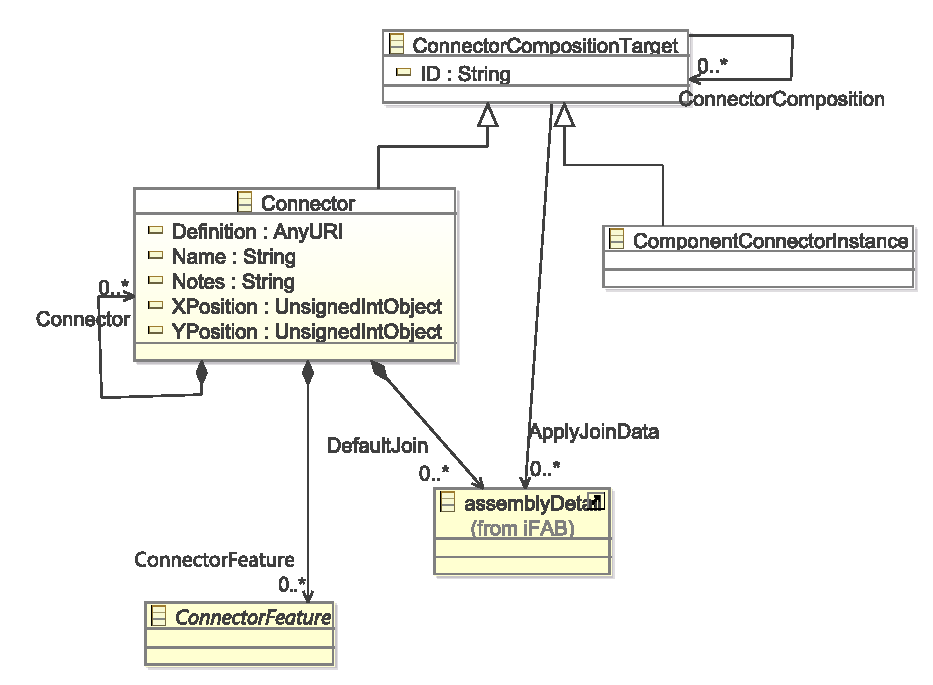
\includegraphics[width=\textwidth]{ClassDiagrams/avm_connector.pdf}}
\caption{avm Namespace: Connector diagram}
\label{Connector_diagram}
\end{figure}

\begin{figure}[h!]
\fbox{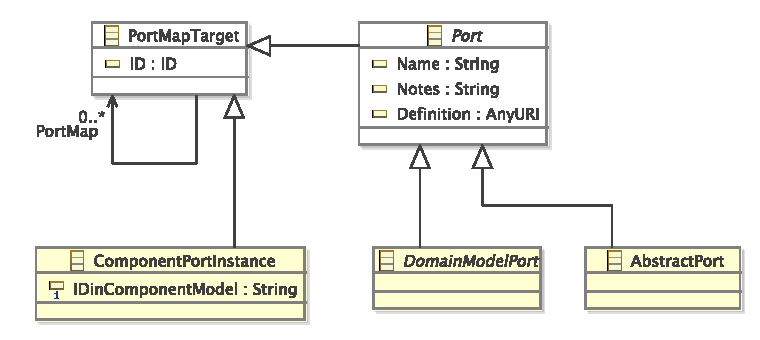
\includegraphics[width=\textwidth]{ClassDiagrams/avm_port.pdf}}
\caption{avm Namespace: Port diagram}
\label{Port_diagram}
\end{figure}


\paragraph{avm.DomainModel}
(Abstract) Baseclass for descriptions of domain-specific models of the component.
\\ \\
\begin{tabular}{ l l p{12cm} }
\textbf{Attribute} & \textbf{Type} & \textbf{Description} \\ \hline
Author & String & The author of the model \\ \hline
Name & String & The name of the model \\ \hline
Notes & String & Any notes regarding the model \\ \hline
XPosition & Unsigned Int & The X Position of the element, if rendered graphically within its parent model \\ \hline
YPosition & Unsigned Int & The Y Position of the element, if rendered graphically within its parent model \\ \hline
\end{tabular}
\\ \\ \\ \\
\begin{tabular}{ l l p{12cm} }
\textbf{Relation} & \textbf{Type} & \textbf{Description} \\ \hline
UsesResource & Resource & Links the DomainModel description to the concrete artifacts implementing the model \\ \hline
\end{tabular}

\paragraph{avm.DomainModelPort}
(Abstract) Baseclass for domain-specific ports contained within Domain Model objects. Since each domain has its own characteristic ports, this concept must be defined for each Domain Model type.
\\ \\
\begin{tabular}{ l l p{12cm} }
\textbf{Attribute} & \textbf{Type} & \textbf{Description} \\ \hline
Notes & String & Any notes regarding the model \\ \hline
XPosition & Unsigned Int & The X Position of the element, if rendered graphically within its parent model \\ \hline
YPosition & Unsigned Int & The Y Position of the element, if rendered graphically within its parent model \\ \hline
\end{tabular}


\paragraph{avm.DomainModelParameter}
(Abstract) Baseclass for parameters of Domain Models. Since each domain may have its own rules about parameters, this concept must be defined for each Domain Model type.
\\ \\
\begin{tabular}{ l l p{12cm} }
\textbf{Attribute} & \textbf{Type} & \textbf{Description} \\ \hline
Notes & String & Any notes regarding the parameter \\ \hline
\end{tabular}

\paragraph{avm.DomainModelMetric}
(Abstract) Baseclass for Metrics of Domain Models. A Metric is a value that can be extracted from the model after it has been used in an analysis. It may be a simulation variable that must be checked after a simulation, the moment-of-inertia of a physical object once it has been parametrically sized, etc.
\\ \\
\begin{tabular}{ l l p{12cm} }
\textbf{Attribute} & \textbf{Type} & \textbf{Description} \\ \hline
ID & ID & The ID of the metric, unique within the scope of the component model \\ \hline
Notes & String & Any notes regarding the metric \\ \hline
XPosition & Unsigned Int & The X Position of the element, if rendered graphically within its parent model \\ \hline
YPosition & Unsigned Int & The Y Position of the element, if rendered graphically within its parent model \\ \hline
\end{tabular}
\\ \\ \\
\begin{tabular}{ l l p{12cm} }
\textbf{Relation} & \textbf{Type} & \textbf{Description} \\ \hline
Value & Value & A Value object capturing the last-calculated value of this metric \\ \hline
\end{tabular}


\begin{figure}[h!]
\fbox{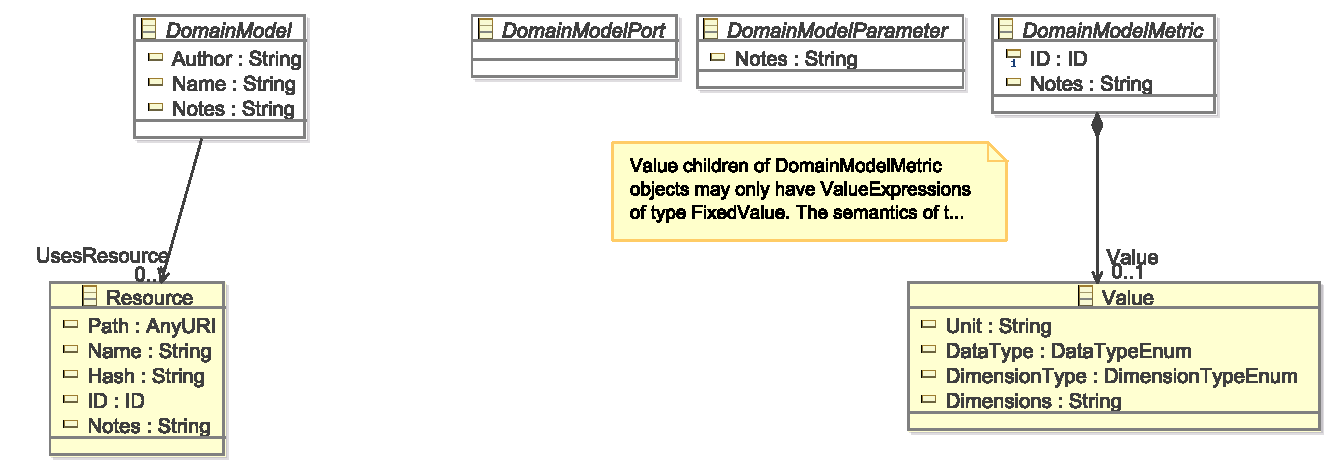
\includegraphics[width=\textwidth]{ClassDiagrams/avm_domainmodel.pdf}}
\caption{avm Namespace: DomainModel diagram}
\end{figure}

\paragraph{avm.Resource}
Describes an artifact that must be included with the Component model, including models used for analysis, documentation, images, etc. Services that process Component models use these links to locate the artifacts with which it is associated.
\\ \\
\begin{tabular}{ l l p{12cm} }
\textbf{Attribute} & \textbf{Type} & \textbf{Description} \\ \hline
Name & AnyURI & A name for this linked Resource \\ \hline
Path & AnyURI & The path to the Resource. May either be an absolute path, or a path relative to the component ACM file itself. \\ \hline
Hash & String & MD5 hash of the artifact \\ \hline
Notes & String & Any notes describing the artifact \\ \hline
ID & ID & The ID of this resource, unique within the scope of the component model \\ \hline
XPosition & Unsigned Int & The X Position of the element, if rendered graphically within its parent model \\ \hline
YPosition & Unsigned Int & The Y Position of the element, if rendered graphically within its parent model \\ \hline
\end{tabular}

\begin{MyVerbatim}
  <ResourceDependency 
    ID="cad_stp.path" 
    Name="h170_cat_c9_600hp_prt.stp" 
    Notes="STEP\H_Power_Package_Drivetrain\h170_cat_c9_600hp_prt.stp" 
    Path="CAD\h170_cat_c9_600hp_prt.stp"/>
\end{MyVerbatim}

\subsubsection{avm.modelica Namespace}

\paragraph{avm.modelica.ModelicaModel}
\textit{Subtype of avm.DomainModel}\\
Describes a Modelica Model of the Component's behavior. Note that this does not \textit{define} a ModelicaModel, it just describes the key features of a Modelica model that is defined in a separate .mo file.
\\ \\
\begin{tabular}{ l l p{9cm} }
\textbf{Attribute} & \textbf{Type} & \textbf{Description} \\ \hline
Class & String & (Required) The full path of the Modelica Model class \\ \hline
\end{tabular}
\\ \\ \\
\begin{tabular}{ l l p{9cm} }
\textbf{Relation} & \textbf{Type} & \textbf{Description} \\ \hline
Connector & avm.modelica.Connector & A child Connector of the model \\ \hline
Parameter & avm.modelica.Parameter & A parameter of the model \\ \hline
Redeclare & avm.modelica.Redeclare & A redeclare statement of the model \\ \hline
Metric & avm.modelica.Metric & A metric of the model \\ \hline
Limit & avm.modelica.Limit & A limit of the model \\ \hline
\end{tabular}

\begin{MyVerbatim}
 <DomainModel 
   Author="Ricardo" 
   Class="C2M2L_Ext.C2M2L_Delivered_Component_Implementations.Prime_Movers.
          Reciprocating.Compression_Ignition.Engine_Basic.
          Example_Engine_Basic_Tstat_Degas" 
   Notes="LanguageVersion:3.2 ModelingTool:Dymola ToolVersion:2013 (64-bit)
          FileFormat:mo" 
   UsesResource="modelica.path" 
   xsi:type="ns3:ModelicaModel">
   ...
 </DomainModel>
\end{MyVerbatim}

\paragraph{avm.modelica.Parameter}
A description of a parameter of a Modelica entity.
\\ \\
\begin{tabular}{ l l p{9cm} }
\textbf{Attribute} & \textbf{Type} & \textbf{Description} \\ \hline
Locator & String & (Required) The path to the parameter, relative to its parent entity \\ \hline
\end{tabular}
\\ \\ \\
\begin{tabular}{ l l p{9cm} }
\textbf{Relation} & \textbf{Type} & \textbf{Description} \\ \hline
Value & Value & Describes the value of the parameter \\ \hline
\end{tabular}

\begin{MyVerbatim}
    <Parameter 
      Locator="mass" 
      Notes="cml_zodb.cml_basic_physicals.Mass">
      <Value ID="mod.Parameter.mass">
        <ValueExpression ValueSource="nv.common_info.mass"  
           xsi:type="ns1:DerivedValue"/>
      </Value>
    </Parameter>
\end{MyVerbatim}

\paragraph{avm.modelica.Metric}
A metric of the Modelica Model.
\\ \\
\begin{tabular}{ l l p{9cm} }
\textbf{Attribute} & \textbf{Type} & \textbf{Description} \\ \hline
Locator & String & (required) The path to the varable to be checked, relative to the parent object. \\ \hline
\end{tabular}

\begin{MyVerbatim}
    <Metric ID="mod.metric.max_top_hose_temp.y" 
      Locator="max_top_hose_temp.y" 
      Notes="cml_zodb.cml_basic_physicals.Temperature"/>
\end{MyVerbatim}

\paragraph{avm.modelica.Limit}
A limit imposed on a variable of the Modelica Model. The value of the variable (or signal) must be checked after a simulation has completed.
\\ \\
\begin{tabular}{ l l p{9cm} }
\textbf{Attribute} & \textbf{Type} & \textbf{Description} \\ \hline
Name & String & The name of the limit \\ \hline
VariableLocator & String & (required) The path to the varable to be checked, relative to the parent of the Limit object \\ \hline
BoundType & BoundTypeEnum & (required) Describes the type of bounded limitation imposed on the variable \\ \hline
ToleranceTimeWindow & Float & The maximum period of time for which it is acceptable for the variable to violate its bounds \\ \hline
Notes & String & Any notes describing the limit \\ \hline
\end{tabular}
\\ \\ \\
\begin{tabular}{ l l p{9cm} }
\textbf{Relation} & \textbf{Type} & \textbf{Description} \\ \hline
TargetValue &Value & Describes the value against which the Limit's bounds must be tested \\ \hline
\end{tabular}

\begin{MyVerbatim}
    <Limit 
      BoundType="MustNotExceed" 
      Name="max_top_hose_temp" 
      VariableLocator="mod.metric.max_top_hose_temp.y">
      <TargetValue>
        <ValueExpression ValueSource="nv.max_top_hose_temp" 
           xsi:type="ns1:DerivedValue"/>
      </TargetValue>
    </Limit>
\end{MyVerbatim}

\paragraph{avm.modelica.Connector}
A description of a Modelica Connector. Note that this concept is distinct from the avm.Connector concept. Connector is a first-class concept within Modelica.
\\ \\
\begin{tabular}{ l l p{9cm} }
\textbf{Attribute} & \textbf{Type} & \textbf{Description} \\ \hline
Class & String & (Required) The full path of the Connector's class \\ \hline
Locator & String & The path to the instantiated Connector, relative to the ModelicaModel in which it is contained \\ \hline
\end{tabular}
\\ \\ \\
\begin{tabular}{ l l p{9cm} }
\textbf{Relation} & \textbf{Type} & \textbf{Description} \\ \hline
Redeclare & avm.modelica.Redeclare & A redeclare statement of the Connector \\ \hline
Parameter & avm.modelica.Parameter & A parameter of the Connector \\ \hline
\end{tabular}

\begin{MyVerbatim}
    <Connector 
      Class="Modelica.Fluid.Interfaces.FluidPort" 
      ID="mod.conn.from_cac" 
      Name="from_cac">
      <Redeclare Locator="Medium" Type="Package">
        <Value>
          <ValueExpression xsi:type="ns1:FixedValue">
            <Value>C2M2L_Ext.Media.Ideal_Gases.Simple_Air</Value>
          </ValueExpression>
        </Value>
      </Redeclare>
    </Connector>
\end{MyVerbatim}

\paragraph{Class Diagrams}
\begin{figure}[h!]
\fbox{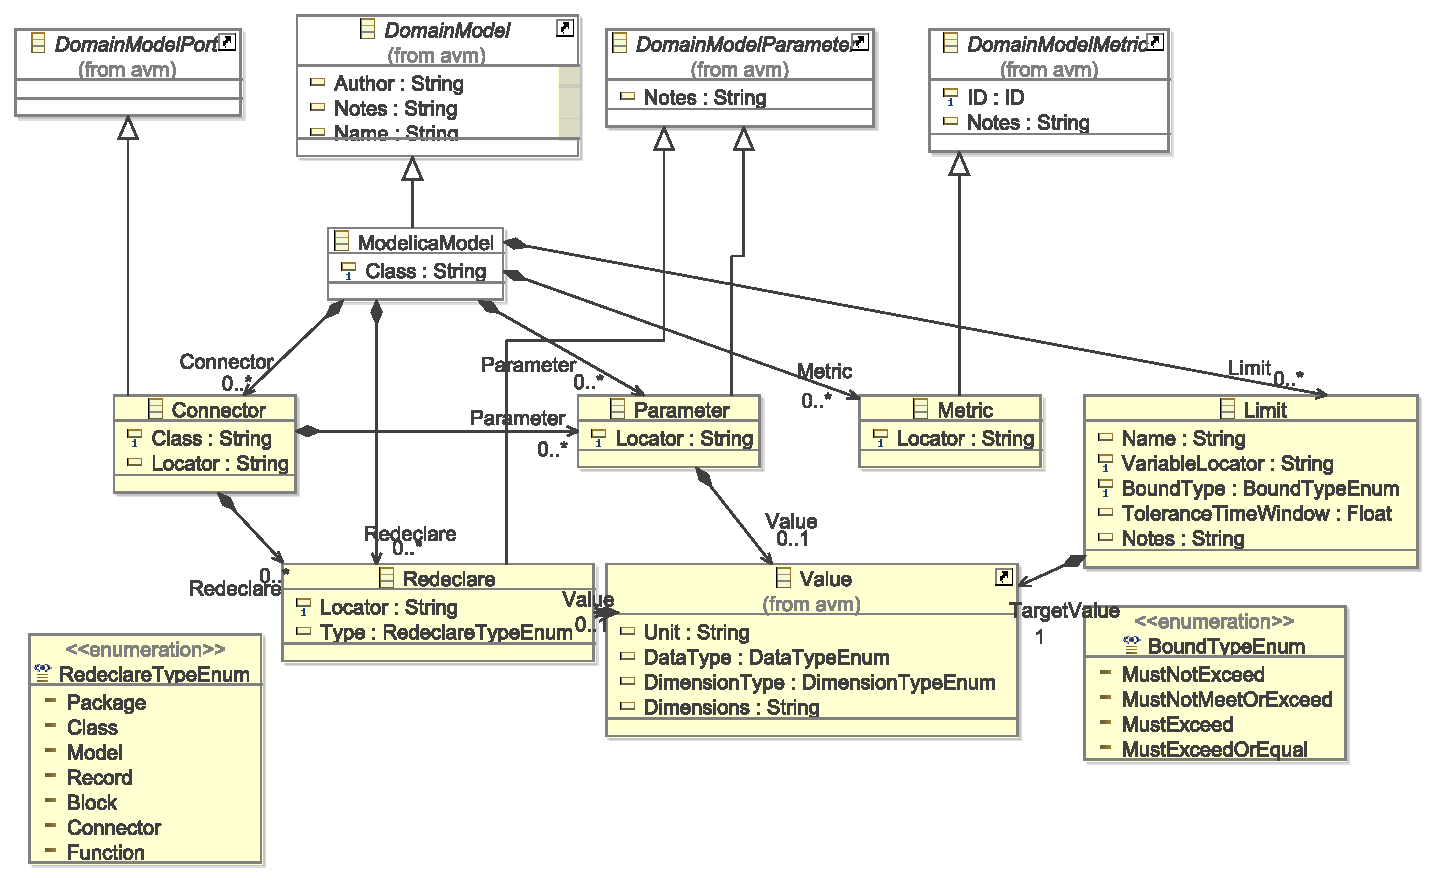
\includegraphics[width=\textwidth]{ClassDiagrams/avm-modelica.pdf}}
\caption{avm.modelica Namespace}
\end{figure}

\begin{figure}[h!]
\fbox{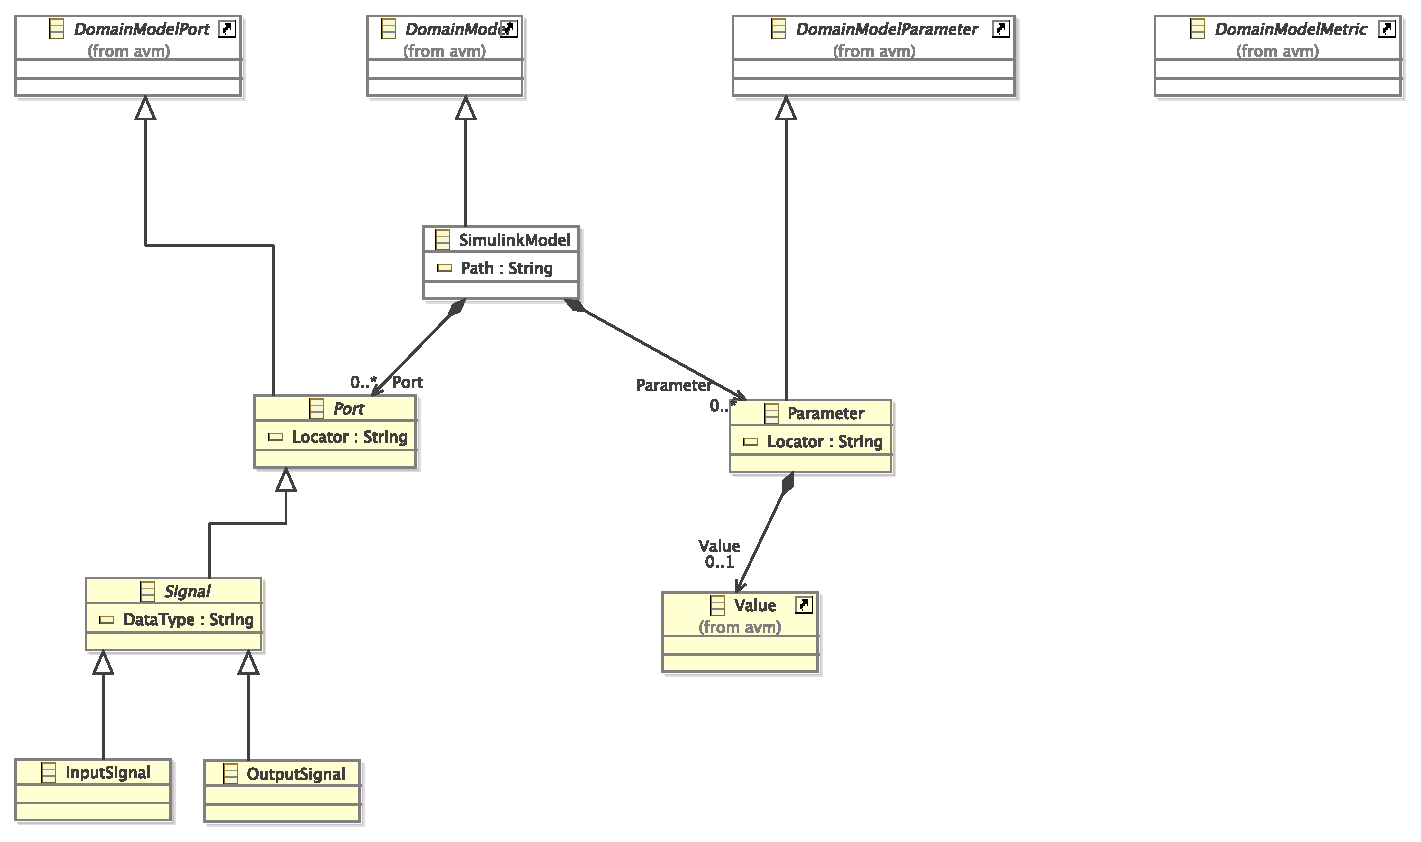
\includegraphics[width=\textwidth]{ClassDiagrams/avm-simulink.pdf}}
\caption{avm.simulink Namespace}
\end{figure}


\subsubsection{avm.cad Namespace}

\paragraph{avm.cad.CADModel}
\textit{Subtype of avm.DomainModel}\\
Describes a CAD Model of the Component. Note that this does not \textit{define} a CAD Model, it just describes the key features of a CAD model that is defined in a separate file.
\\ \\
\begin{tabular}{ l l p{9cm} }
\textbf{Relation} & \textbf{Type} & \textbf{Description} \\ \hline
Datum & avm.cad.Datum & Describes a Datum in the CAD Model. \\ \hline
Parameter & avm.cad.Parameter & Describes a Parameter of the CAD Model. \\ \hline
ModelMetric & avm.cad.Metric & Describes a Metric in the CAD Model. \\ \hline
\end{tabular}

\begin{MyVerbatim}
 <DomainModel UsesResource="cad.path" xsi:type="ns4:CADModel">
\end{MyVerbatim}

\paragraph{avm.cad.Parameter}
Represents a parameter of the CAD Model file.
\\ \\
\begin{tabular}{ l l p{11cm} }
\textbf{Attribute} & \textbf{Type} & \textbf{Description} \\ \hline
Name & String & (required) The name of the parameter in the CAD Model file. \\ \hline
\end{tabular}
\\ \\ \\
\begin{tabular}{ l l p{11cm} }
\textbf{Relation} & \textbf{Type} & \textbf{Description} \\ \hline
Value & Value & Describes the value of the parameter. \\ \hline
\end{tabular}

\paragraph{avm.cad.Metric}
A Metric is a property of the CAD Model or Datum that should be retrieved and set once the model has been used in a system composition.
Common applications include checking the moment of inertia or mass, as calculated by the CAD tool, of a parametrically-variable model, where these values are not known until the parameter values are applied.
\\ \\
\begin{tabular}{ l l p{11cm} }
\textbf{Attribute} & \textbf{Type} & \textbf{Description} \\ \hline
Name & String & (required) The name of the property in the CAD Model file. \\ \hline
\end{tabular}

\begin{MyVerbatim}
   <ModelMetric ID="cad.TOTAL_MASS" Name="TOTAL_MASS">
      <Value DataType="Integer" DimensionType="Scalar" Dimensions="1" 
        ID="cad.value.TOTAL_MASS" Unit="kg">
        <ValueExpression xsi:type="ns1:FixedValue">
          <Value>898</Value>
        </ValueExpression>
      </Value>
    </ModelMetric>
\end{MyVerbatim}

\paragraph{avm.cad.Datum}
(Abstract) Describes a Datum that can be found in the CAD Model. Note that this does not \textit{define} a Datum, it just describes one that can be found in the CAD Model.
\\ \\
\begin{tabular}{ l l p{9cm} }
\textbf{Attribute} & \textbf{Type} & \textbf{Description} \\ \hline
DatumName & String & The name of the datum in the CAD Model file. \\ \hline
\end{tabular}
\\ \\ \\
\begin{tabular}{ l l p{9cm} }
\textbf{Relation} & \textbf{Type} & \textbf{Description} \\ \hline
DatumMetric & avm.cad.Metric & Describes a Metric of the Datum. \\ \hline
\end{tabular}

\paragraph{avm.cad.Point}
\textit{Subtype of avm.cad.Datum}\\
Represents a Point datum within the CAD Model file.

\paragraph{avm.cad.Axis}
\textit{Subtype of avm.cad.Datum}\\
Represents an Axis datum within the CAD Model file.

\begin{MyVerbatim}
    <Datum DatumName="EXT_MOUNT_1_axis_z" 
      ID="cad.EXT_MOUNT_1_axis_z" 
      xsi:type="ns4:Axis"/>
\end{MyVerbatim}

\paragraph{avm.cad.Plane}
\textit{Subtype of avm.cad.Datum}\\
Represents a Plane datum within the CAD Model file.
\\ \\ \\
\begin{tabular}{ l l p{9cm} }
\textbf{Relation} & \textbf{Type} & \textbf{Description} \\ \hline
SurfaceReverseMap & avm.cad.Plane & Used for mapping a Plane datum to a corresponding Role in a Connector. An alternative to PortMap, this relation will reverse the Side A - Side B matching semantics from the usual case. \\ \hline
\end{tabular}

\begin{MyVerbatim}
    <Datum DatumName="EXT_MOUNT_1_plane_xy" 
      ID="cad.EXT_MOUNT_1_plane_xy" 
      xsi:type="ns4:Plane"/>
\end{MyVerbatim}

\paragraph{avm.cad.CoordinateSystem}
\textit{Subtype of avm.cad.Datum}\\
Represents a Coordinate System datum within the CAD Model file.

\paragraph{avm.cad.GuideDatum}
\textit{Subtype of avm.ConnectorFeature}\\
A \textbf{Guide Datum} is a marker that modifies the meaning of a datum. Whereas typically Datums from composed Connectors are constrained permanently in a CAD model, Guide Datums are constrained only while the model is being constructed, and are then unconstrained once the model is complete. If a composition is underconstrained, as in a joint, the Guide Datums may be used to set an "initial position" for the two parts.

\begin{tabular}{ l l p{9cm} }
\textbf{Relation} & \textbf{Type} & \textbf{Description} \\ \hline
Datum & avm.cad.Datum & Maps to the ID of the datum that should be considered a Guide Datum. \\ \hline
\end{tabular}

\begin{MyVerbatim}
    <Datum DatumName="EXT_TORQUE_OUT" 
      Definition="CML_Mapping\cml_zodb.cml_extended_physicals.Coord_System_Definition" 
      ID="cad.EXT_TORQUE_OUT" 
      xsi:type="ns4:CoordinateSystem">
      <Metric ID="cad.EXT_TORQUE_OUT.position" Name="position">
        <Value DimensionType="Vector" 
          ID="cad.EXT_TORQUE_OUT.position.vector" Unit="mm">
          <ValueExpression xsi:type="ns1:FixedValue">
            <Value>{0.0,2.35408792633e-18,-0.06825}</Value>
          </ValueExpression>
        </Value>
      </Metric>
      <Metric ID="cad.EXT_TORQUE_OUT.local_x" Name="local_x">
        <Value DimensionType="Vector" 
          ID="cad.EXT_TORQUE_OUT.local_x.vector" Unit="mm">
          <ValueExpression xsi:type="ns1:FixedValue">
            <Value>{1.0,0.0,0.0}</Value>
          </ValueExpression>
        </Value>
      </Metric>
      <Metric ID="cad.EXT_TORQUE_OUT.local_y" Name="local_y">
        <Value DimensionType="Vector" 
          ID="cad.EXT_TORQUE_OUT.local_y.vector" Unit="mm">
          <ValueExpression xsi:type="ns1:FixedValue">
            <Value>{0.0,1.0,0.0}</Value>
          </ValueExpression>
        </Value>
      </Metric>
    </Datum>
\end{MyVerbatim}

\paragraph{Class Diagrams}
\begin{figure}[h!]
\fbox{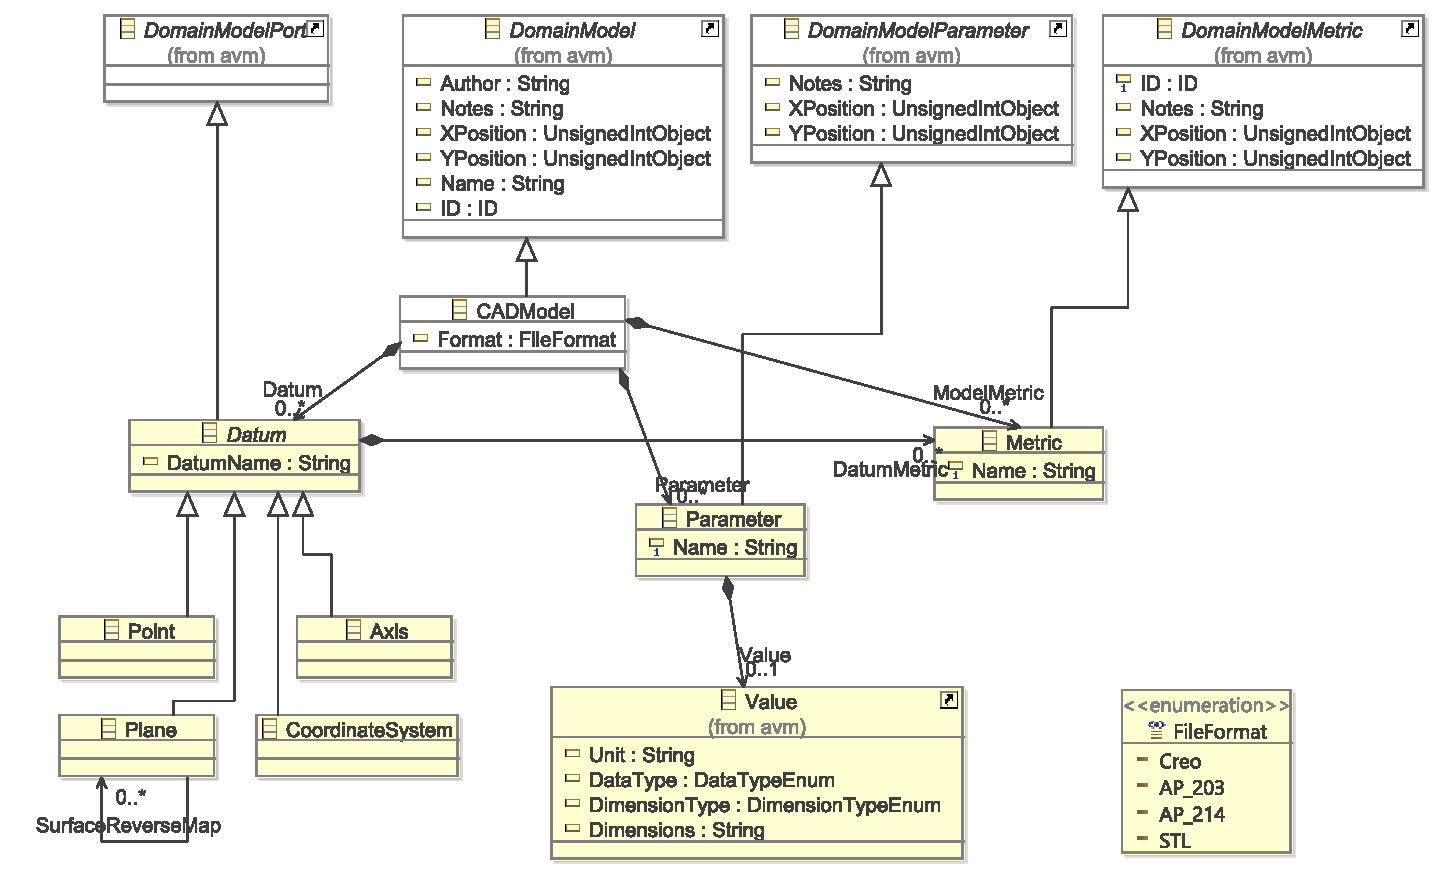
\includegraphics[width=\textwidth]{ClassDiagrams/avm-cad_cadmodel.pdf}}
\caption{avm.cad Namespace: CADModel diagram}
\end{figure}

\begin{figure}[h!]
\fbox{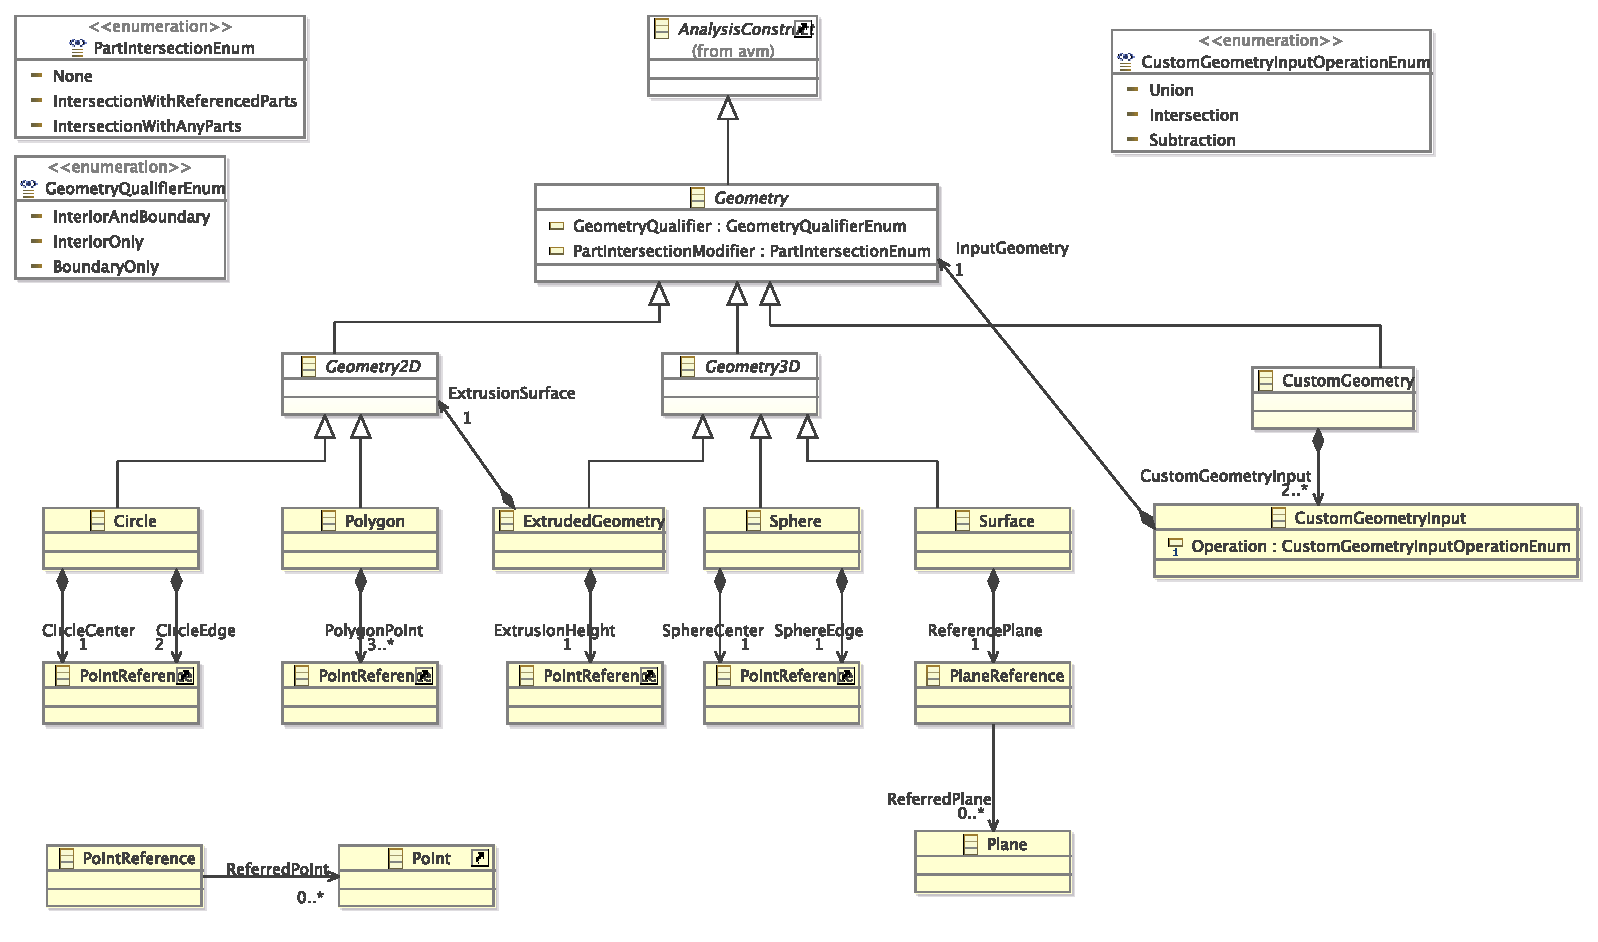
\includegraphics[width=\textwidth]{ClassDiagrams/avm-cad_geometry.pdf}}
\caption{avm.cad Namespace: Geometry diagram}
\end{figure}

\begin{figure}[h!]
\fbox{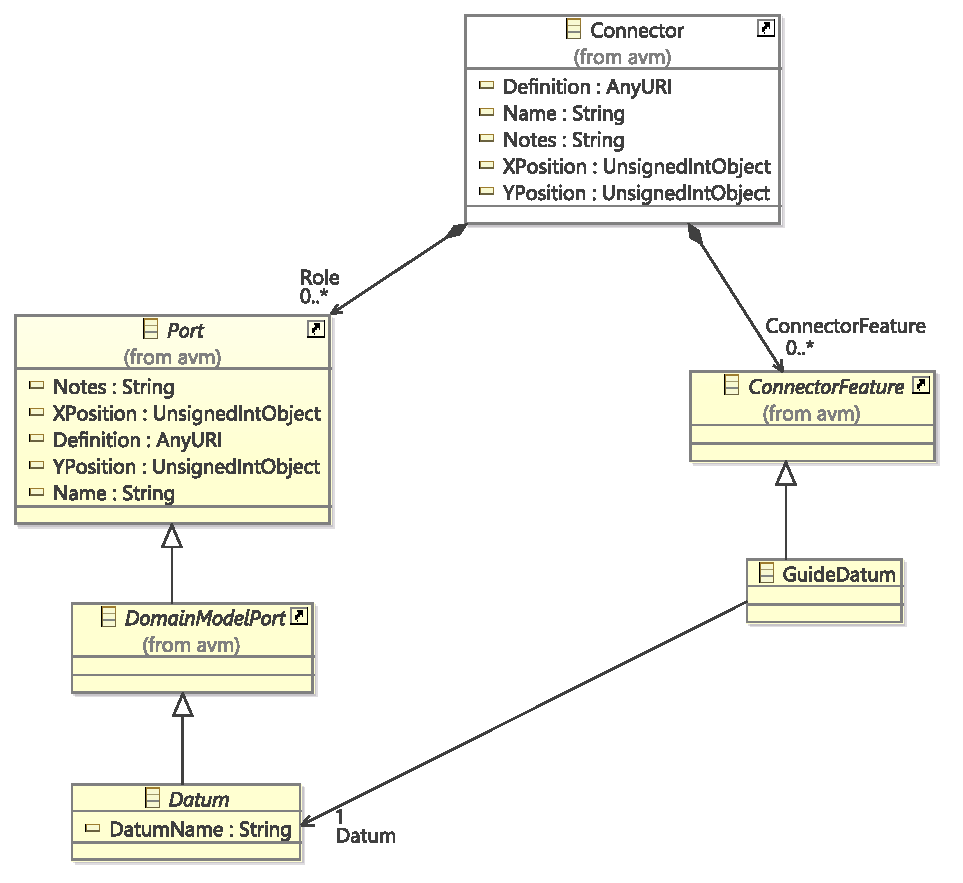
\includegraphics[width=\textwidth]{ClassDiagrams/avm-cad_guidedatum.pdf}}
\caption{avm.cad Namespace: Guide Datum diagram}
\end{figure}

\subsubsection{avm.manufacturing Namespace}
\begin{figure}[h!]
\fbox{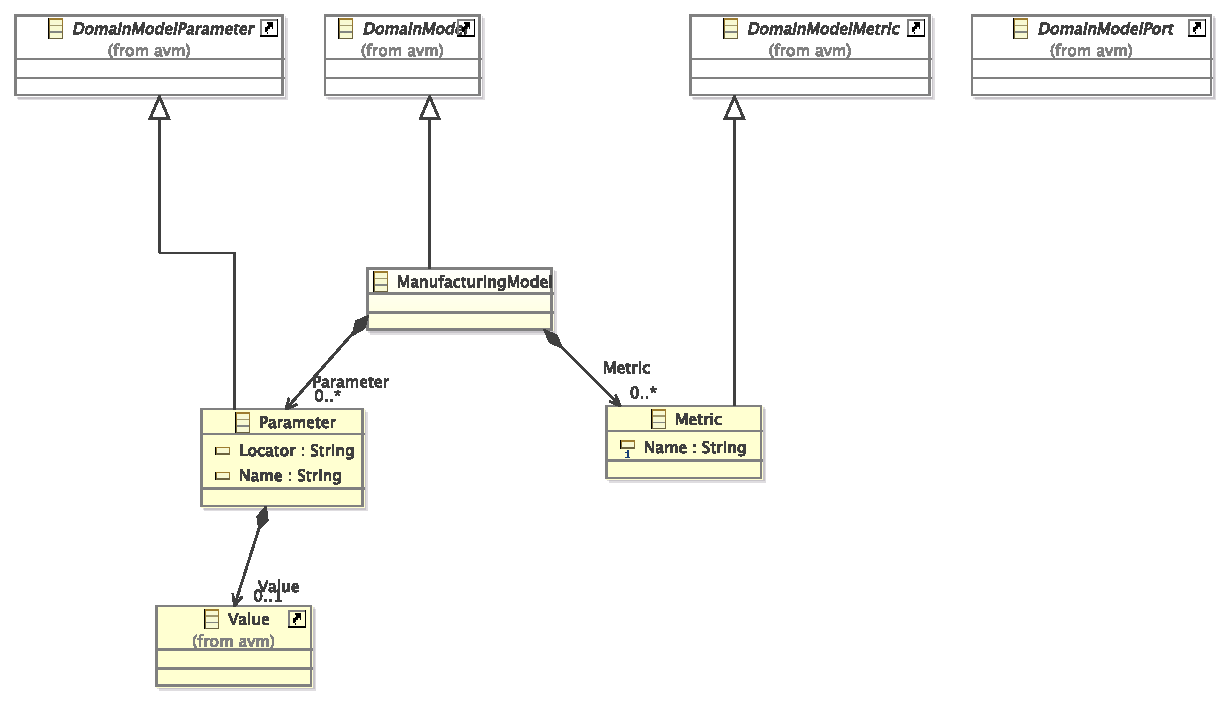
\includegraphics[width=\textwidth]{ClassDiagrams/avm-manufacturing.pdf}}
\caption{avm.manufacturing Namespace}
\end{figure}

\paragraph{avm.manufacturing.ManufacturingModel}
\textit{Subtype of avm.DomainModel}\\
Describes a Manufacturing Model of the Component.
Note that this does not \textit{define} a Manufacturing Model, it just describes the key features of a Manufacturing model that is defined in a separate file.
\\ \\
\begin{tabular}{ l l p{9cm} }
\textbf{Relation} & \textbf{Type} & \textbf{Description} \\ \hline
Parameter & avm.manufacturing.Parameter & Describes a parameter of the Manufacturing model. \\ \hline
Metric & avm.manufacturing.Metric & Describes a metric of the Manufacturing model. \\ \hline
\end{tabular}

\begin{MyVerbatim}
  <DomainModel UsesResource="manuf.path" 
    xsi:type="ns2:ManufacturingModel">
\end{MyVerbatim}

\paragraph{avm.manufacturing.Parameter}
Describes a parameter of the Manufacturing model.
\\ \\
\begin{tabular}{ l l p{11cm} }
\textbf{Attribute} & \textbf{Type} & \textbf{Description} \\ \hline
Locator & String & The path to the corresponding field in the Manufacturing Model. \\ \hline
Name & String & A user-friendly name for this parameter. \\ \hline
\end{tabular}
\\ \\ \\
\begin{tabular}{ l l p{11cm} }
\textbf{Relation} & \textbf{Type} & \textbf{Description} \\ \hline
Value & Value & Describes the value of the parameter. \\ \hline
\end{tabular}

\begin{MyVerbatim}
    <Parameter Name="procurement__make_or_buy">
      <Value DataType="String" DimensionType="Scalar" Dimensions="1" 
        ID="procurement.make_or_buy">
        <ValueExpression xsi:type="ns1:FixedValue">
          <Value>Buy</Value>
        </ValueExpression>
      </Value>
    </Parameter>
\end{MyVerbatim}

\paragraph{avm.manufacturing.Metric}
Describes a Metric of the Manufacturing model. This is a value that must be calculated by an analysis tool, such as the per-unit cost for a fabricated component.
\\ \\
\begin{tabular}{ l l p{9cm} }
\textbf{Attribute} & \textbf{Type} & \textbf{Description} \\ \hline
Name & String & (required) The name of the property to be extracted. \\ \hline
\end{tabular}

\subsection{Restrictions}
Although many restrictions on model structure are imposed by the XML Schema (XSD), not all are currently checked. This section lists some of the additional restrictions.

\subsubsection{Property Names}
Each Property must have a unique name within its level of hierarchy.

Property names must conform to the limitations of Modelica names, and not include the following characters (among others): 
\begin{verbatim}
. / \
\end{verbatim}

\subsubsection{Property Values}
All Property objects must have a Value child.

\subsection{ComplexFormula Expression Syntax}
\label{subsec:ComplexFormulaExpressionSyntax}
\textbf{ComplexFormula} objects contain \textit{Expression}s which allow mathematical formulas to be defined. These expressions must use the syntax defined by the \textbf{MuParser} math library. The resulting value of such an \textit{Expression} is considered to be the value of the \textbf{CustomFormula} node, so no assignment operator is required. Note that only a subset of MuParser syntax is supported. Supported functions and operators are listed here. The original documentation for MuParser's syntax can be found here: \url{http://muparser.beltoforion.de/mup_features.html#idDef2}
\\ \\
In \textbf{ComplexFormula} \textit{Expression}s, model-defined \textbf{operands} can be referenced using their \textit{Symbol}s.

\subsubsection{Functions}
\begin{tabular}{ l }
\textbf{Function} \\ \hline
sin(x) \\ \hline
cos(x) \\ \hline
tan(x) \\ \hline
asin(x) \\ \hline
acos(x) \\ \hline
atan(x) \\ \hline
sinh(x) \\ \hline
cosh(x) \\ \hline
tanh(x) \\ \hline
asinh(x) \\ \hline
acosh(x) \\ \hline
atanh(x) \\ \hline
log2(x) \\ \hline
log10(x) \\ \hline
log(x) \\ \hline
ln(x) \\ \hline
exp(x) \\ \hline
sqrt(x) \\ \hline
sign(x) \\ \hline
rint(x) \\ \hline
abs(x) \\ \hline
min(x1, x2, x3, ...) \\ \hline
max(x1, x2, x3, ...) \\ \hline
sum(x1, x2, x3, ...) \\ \hline
avg(x1, x2, x3, ...) \\ \hline
\end{tabular}

\subsubsection{Operators}
Operators with higher priority will be evaluated first.
\\ \\
\begin{tabular}{ l l l }
\textbf{Operator} & \textbf{Meaning} & \textbf{Priority} \\ \hline
\&\& & logical and & 1 \\ \hline
|| & logical or & 2 \\ \hline
\textless= & less or equal & 4 \\ \hline
\textgreater= & greater or equal & 4 \\ \hline
!= & not equal & 4 \\ \hline
== & equal & 4 \\ \hline
\textgreater & greater than & 4 \\ \hline
\textless & less than & 4 \\ \hline
+ & addition & 5 \\ \hline
- & subtraction & 5 \\ \hline
* & multiplication & 6 \\ \hline
/ & division & 6 \\ \hline
\textasciicircum & raise x to the power of y & 7 \\ \hline
\end{tabular}

%\subsection{Sample ACM File}
%The following XML was generated using \textit{test\_builder.py}, included with the Python library.
%
%\definecolor{gray}{rgb}{0.4,0.4,0.4}
%\definecolor{darkblue}{rgb}{0.0,0.0,0.6}
%\definecolor{red}{rgb}{0.6,0.0,0.0}
%
%\lstloadlanguages{XML}
%
%\lstdefinestyle{listXML}{language=XML, extendedchars=true,  belowcaptionskip=5pt, xleftmargin=1.8em, xrightmargin=0.5em, breaklines=true, breakatwhitespace=true, breakindent=0pt, emph={}, emphstyle=\color{red}, basicstyle=\small\ttfamily, columns=fullflexible, showstringspaces=false, commentstyle=\color{gray}\upshape,
%morestring=[b]",
%morecomment=[s]{<?}{?>},
%morecomment=[s][\color{orange}]{<!--}{-->},
%keywordstyle=\color{red},
%stringstyle=\color{black},
%tagstyle=\color{darkblue},
%morekeywords={xmlns,version,type}
%}
%
%\lstinputlisting
%[style=listXML,breaklines=true,tabsize=1,showspaces=false,showstringspaces=false,language=XML,basicstyle=\ttfamily\scriptsize]
%{../exampleprojects/python/python_test_out.acm}
%
%\newpage





\end{document}